%%%%%%%%%%%%%%%%%%%%%%%%%%%%%%%%%%%%%%%%%%%%%%%%%%%%%%%%%%%%
%%% LIVECOMS ARTICLE TEMPLATE FOR BEST PRACTICES GUIDE
%%% ADAPTED FROM ELIFE ARTICLE TEMPLATE (8/10/2017)
%%%%%%%%%%%%%%%%%%%%%%%%%%%%%%%%%%%%%%%%%%%%%%%%%%%%%%%%%%%%
%%% PREAMBLE
\documentclass[9pt,tutorial]{livecoms}
% Use the 'onehalfspacing' option for 1.5 line spacing
% Use the 'doublespacing' option for 2.0 line spacing
% Use the 'lineno' option for adding line numbers.
% Use the 'pubversion' option for adding the citation and publication information to the document footer, when the DOI is assigned and the article is added to a live issue.
% The 'bestpractices' option for indicates that this is a best practices guide.
% Omit the bestpractices option to remove the marking as a LiveCoMS paper.
% Please note that these options may affect formatting.

\usepackage[T1]{fontenc}
\usepackage[utf8]{inputenc}
\usepackage{lmodern}
\usepackage{verbatim}
\usepackage{graphicx}
\usepackage{amsmath}
\usepackage{amssymb}
\usepackage{amsthm}
\usepackage{tabularx}
\usepackage{multirow}
\usepackage{multicol}
\usepackage{fancyvrb}
\usepackage{float}
\usepackage{listings}
\usepackage{xcolor}
\usepackage{array}
\usepackage{booktabs}
\usepackage{times}
\usepackage{subcaption}
\usepackage{mathtools}
\usepackage{microtype}
\usepackage{tcolorbox}
\usepackage{newverbs}
\usepackage{listings}

\usepackage[
    type={CC},
    modifier={by-nc-sa},
    version={4.0},
]{doclicense}

\usepackage{wrapfig}
\usepackage{geometry}

\usepackage[version=4]{mhchem}
\usepackage{siunitx}
\DeclareSIUnit\Molar{M}
\usepackage[italic]{mathastext}
\graphicspath{{figures/}}

\definecolor{mylightblue}{RGB}{68.085,183.09,194.055} 
\definecolor{mystrongblue}{RGB}{2.04,74.97,121.89}
\definecolor{myorange}{RGB}{255.0,173.91,72.93}
\definecolor{graytitle}{gray}{0.5}
\definecolor{cverbbg}{gray}{0.93}

%%%%%%%%%%%%%%%%%%%%%%%%%%%%%%%%%%%%%%%%%%%%%%%%%%%%%%%%%%%%
%%% IMPORTANT USER CONFIGURATION
%%%%%%%%%%%%%%%%%%%%%%%%%%%%%%%%%%%%%%%%%%%%%%%%%%%%%%%%%%%%

\newcommand{\versionnumber}{1.0}  % you should update the minor version number in preprints and major version number of submissions.
% Do not add a newline in the next command, no matter how long the repository name is, as it will break the link in the PDF.
\newcommand{\githubrepository}{\url{https://github.com/lammpstutorials/lammpstutorials-article}}  %this should be the main github repository for this article

%%%%%%%%%%%%%%%%%%%%%%%%%%%%%%%%%%%%%%%%%%%%%%%%%%%%%%%%%%%%
%%% ARTICLE SETUP
%%%%%%%%%%%%%%%%%%%%%%%%%%%%%%%%%%%%%%%%%%%%%%%%%%%%%%%%%%%%
\title{A Suite of Tutorials for the LAMMPS Simulation Package [Article v\versionnumber]}

\author[1*]{Simon Gravelle}
\affil[1]{University Grenoble Alpes, CNRS, LIPhy, Grenoble, 38000, France}

\corr{simon.gravelle@cnrs.fr}{SG}

\orcid{Simon Gravelle}{0000-0003-2149-6706}

\blurb{This LiveCoMS document is maintained online on GitHub at \githubrepository; to provide feedback, suggestions, or help improve it, please visit the GitHub repository and participate via the issue tracker.}

%%%%%%%%%%%%%%%%%%%%%%%%%%%%%%%%%%%%%%%%%%%%%%%%%%%%%%%%%%%%
%%% PUBLICATION INFORMATION
%%% Fill out these parameters when available
%%% These are used when the "pubversion" option is invoked
%%%%%%%%%%%%%%%%%%%%%%%%%%%%%%%%%%%%%%%%%%%%%%%%%%%%%%%%%%%%
\pubDOI{10.XXXX/YYYYYYY}
\pubvolume{<volume>}
\pubissue{<issue>}
\pubyear{<year>}
\articlenum{<number>}
\datereceived{Day Month Year}
\dateaccepted{Day Month Year}

%%%%%%%%%%%%%%%%%%%%%%%%%%%%%%%%%%%%%%%%%%%%%%%%%%%%%%%%%%%%
%%% ARTICLE START
%%%%%%%%%%%%%%%%%%%%%%%%%%%%%%%%%%%%%%%%%%%%%%%%%%%%%%%%%%%%

\begin{document}

\begin{frontmatter}
\maketitle

\begin{abstract}
This particular document provides a skeleton illustrating key sections for a Tutorial document.
Please see the sample \texttt{sample-document.tex} in \url{github.com/livecomsjournal/article_templates/templates} for additional information on and examples of using the LiveCoMS LaTeX class.
Here we also assume familiarity with LaTeX and knowledge of how to include figures, tables, etc.; if you want examples, see the sample just referenced.

In your work, in this particular slot, please provide an abstract of no more than 250 words.
Your abstract should explain the main contributions of your article, and should not contain any material that is not included in the main text.
Please note that your abstract, plus the authorship material following it, must not extend beyond the title page or modifications to the LaTeX class will likely be needed.
\end{abstract}

\end{frontmatter}




\section{Introduction}

Here you would explain what problem you are tackling and briefly motivate your work.

In this particular template, we have removed most of the usage examples which occur in \texttt{sample-document.tex} to provide a minimal template you can modify; however, we retain a couple of examples illustrating more unusual features of our templates/article class, such as the checklists, and information on algorithms and pseudocode.

Keep in mind, as you prepare your manuscript, that you should plan for a representative image  which will be used to highlight your article on the journal website and publications. Usually, this would be one of your figures, but it must also be uploaded separately upon article submission. We give specific guidelines for this image on the journal website in the section on article submission (see \url{https://livecomsjournal.github.io/authors/policies/index.html#article-submission}).

Additionally, for well-formatted manuscripts, we recommend that you let LaTeX handle figure/table placement for you as much as possible, so please avoid specifying strenuous float instructions like `[h!]` and `[H]` as much as possible.

\subsection{Scope}

Tutorials should endeavor to cover the specific task at hand, and also highlight how the steps might need to be modified (or additional care might need to be taken at particular points) to handle more general cases.

The scope of the tutorial, as well as the expected proficiencies / outcomes for researchers who complete the tutorial, should be clearly defined.
This will often happen in a specific section or subsection in the article itself.

\section{Prerequisites}

Here you would identify prerequisites/background knowledge that are assumed by your work, as well as any software/license requirements.

\subsection{Background knowledge}
Tutorials should clearly define what concepts or abilities researchers will need to complete the tutorial (e.g., some proficiency in Python; experience with Jupyter notebooks; knowledge of classical MD; etc).

\subsection{Software/system requirements}
Tutorials should clearly define what system and/or software requirements the researcher will need to complete the tutorial (e.g., VMD version 1.9 or newer, AMBER, etc.). Tutorials requiring specific software packages must provide instructions and files for the referenced version of the software.

\section{Content and links}

A tutorial will normally draw on additional files and materials; clearly indicate where and how these are available, with links, and how they are being archived for the long-term and maintained so they stay current.
You will likely want to reference your GitHub repository as a central point to access all of this information, and then the GitHub repository may link out to other content as needed.

\subsection{Tutorial 1: Lennard-Jones fluid}
\label{lennard-jones-label}

\begin{figure}
{\centering
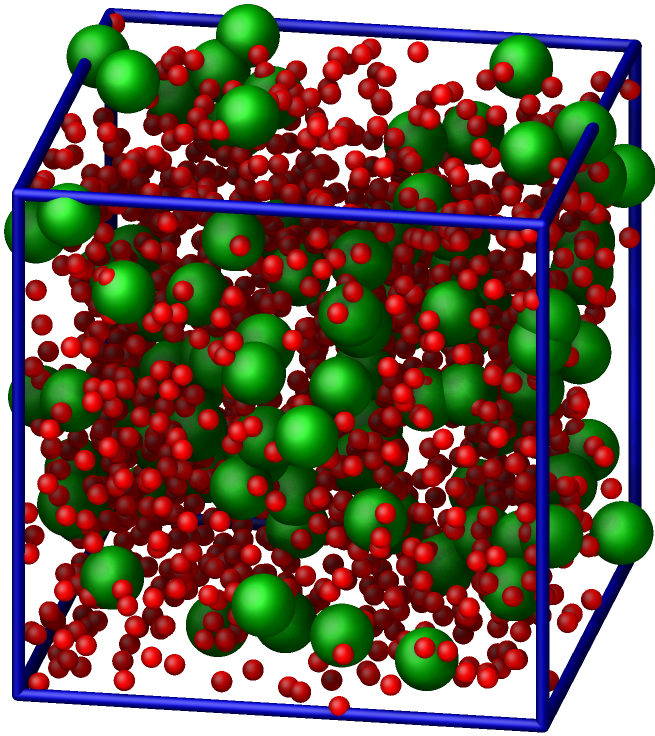
\includegraphics[width=0.55\linewidth]{LJ}
\caption{Snapshot of the Lennard-Jones fluid made using VMD, with both types of atoms represented as spheres.}}
\label{fig:binary_LJ_fluid}
\end{figure}

\noindent The objective of this tutorial is to perform the simulation of a binary fluid using LAMMPS. The system is a Lennard-Jones fluid made of neutral particles with two different diameters in a cubic box with periodic boundary conditions (Fig.~\ref{fig:binary_LJ_fluid}). The temperature of the system is maintained using a Langevin thermostat \cite{schneider1978molecular}, and basic quantities are extracted from the system, including the potential and kinetic energies. 

\subsubsection{My first input}

\noindent To run a simulation using LAMMPS, one needs to write a series of commands in an input script. For clarity, this script will be divided into five categories which we are going to fill up one by one. Create a folder, call it \textit{my-first-input/}, and then create a blank text file in it called \textit{input.lammps}. Copy the following lines in \textit{input.lammps}, where a line starting with a brace ($\#$) is a comment that is ignored by LAMMPS:
{\small \begin{verbatim}
# PART A - ENERGY MINIMIZATION
# 1) Initialization
# 2) System definition
# 3) Simulation settings
# 4) Visualization
# 5) Run
\end{verbatim}}
\noindent These five categories are not required in every input script, and should not necessarily be in that exact order. For instance, parts 3 and 4 could be inverted, or part 4 could be omitted. Note however that LAMMPS reads input files from top to bottom, therefore the \textit{Initialization} and \textit{System definition} categories must appear at the top of the input, and the \textit{Run} category at the bottom.

\paragraph{System initialization}
In the first section of the script, called \textit{Initialization}, let us indicate to LAMMPS the most basic information about the simulation, such as:
\begin{itemize}
\item the conditions at the boundaries of the box (e.g. periodic or non-periodic),
\item the type of atoms (e.g. uncharged single dots or spheres with angular velocities).
\end{itemize}
Enter the following lines in \textit{input.lammps}:
{\small \begin{verbatim}
# 1) Initialization
units lj
dimension 3
atom_style atomic
pair_style lj/cut 2.5
boundary p p p
\end{verbatim}}
The first line, \textit{units lj}, indicates that we want to use the system of unit called \textit{LJ}, for Lennard-Jones, for which all quantities are unitless. The second line, \textit{dimension 3}, indicates that the simulation is 3D. The third line, \textit{atom$\_$style atomic}, that the \textit{atomic} style
will be used, therefore each atom is just a dot with a mass. The fourth line, \textit{pair$\_$style lj/cut 2.5}, indicates that atoms will be interacting through a Lennard-Jones potential with a cut-off equal to $r_c = 2.5$ (unitless) \cite{wang2020lennard,fischer2023history}:
$$E_{ij} (r) = 4 \epsilon_{ij} \left[ \left( \dfrac{\sigma_{ij}}{r} \right)^{12} - \left( \dfrac{\sigma_{ij}}{r} \right)^{6} \right], ~ \text{for} ~ r < r_c,$$
where $r$ is the inter-particles distance, $\epsilon_{ij}$ the depth of potential well that sets the interaction strength, and $\sigma_{ij}$ the distance parameter, or particle effective size. Here, the indexes \textit{ij} refer to the particle types \textit{i} and \textit{j}. The last line, \textit{boundary p p p}, indicates that the periodic boundary conditions will be used along all three directions of space (the 3 \textit{p} stand for \textit{x}, \textit{y}, and \textit{z}, respectively).

\paragraph{System definition}
Let us fill the \textit{System definition} category of the input script:
{\small \begin{verbatim}
# 2) System definition
region simulation_box block -20 20 -20 20 -20 20
create_box 2 simulation_box
create_atoms 1 random 1500 341341 simulation_box
create_atoms 2 random 100 127569 simulation_box
\end{verbatim}}
\noindent The first line, \textit{region simulation$\_$box (...)}, creates a region named \textit{simulation$\_$box} that is a block (i.e. a rectangular cuboid) that extends from -20 to 20 (no unit) along all 3 directions of space. The second line, \textit{create$\_$box 2 simulation$\_$box}, creates a simulation box based on the region \textit{simulation$\_$box} with \textit{2} types of atoms. The third line, \textit{create$\_$atoms (...)} creates 1500 atoms of type 1 randomly within the region \textit{simulation$\_$box}. The integer \textit{341341} is a seed that can be changed in order to create different
initial conditions for the simulation. The fourth line creates 100 atoms of type 2.

\paragraph{Simulation Settings}
Let us fill the \textit{Simulation Settings} category section of the \textit{input} script:
{\small \begin{verbatim}
# 3) Simulation settings
mass 1 1
mass 2 1
pair_coeff 1 1 1.0 1.0
pair_coeff 2 2 0.5 3.0
\end{verbatim}}
The two first commands, \textit{mass (...)}, attribute a mass equal to 1 (unitless) to both atoms of type 1 and 2. Alternatively, one could have written these two commands into one single line: \textit{mass $\star 1$}, where the star symbol means \textit{all} the atom types of the simulation.  The third line, \textit{pair$\_$coeff 1 1 1.0 1.0}, sets the Lennard-Jones coefficients for the interactions between atoms of type 1, respectively the energy parameter $\epsilon_{11} = 1.0$ and the distance parameter $\sigma_{11} = 1.0$. Similarly, the last line sets the Lennard-Jones coefficients for the interactions between atoms of type 2, $\epsilon_{22} = 0.5$, and $\sigma_{22} = 3.0$. By default, LAMMPS calculates the cross coefficients between the different atom types using geometric average: $\epsilon_{ij} = \sqrt{\epsilon_{ii} \epsilon_{jj}}$, $\sigma_{ij} = \sqrt{\sigma_{ii} \sigma_{jj}}$. 

\paragraph{Energy minimization}
The system is now fully parametrized. Let us fill the two last remaining sections by adding the following lines to \textit{input.lammps}:
{\small \begin{verbatim}
# 4) Visualization
thermo 10
thermo_style custom step temp pe ke etotal press

# 5) Run
minimize 1.0e-4 1.0e-6 1000 10000
\end{verbatim}}
The \textit{thermo} command asks LAMMPS to print thermodynamic information (e.g. temperature, energy) in the terminal every given number of steps, here 10 steps. The \textit{thermo$\_$style custom} requires LAMMPS to print the system temperature (\textit{temp}), potential energy (\textit{pe}), kinetic energy (\textit{ke}), total energy (\textit{etotal}), and pressure (\textit{press}). Finally, the \textit{minimize} line asks LAMMPS to perform an energy minimization of the system. By default, LAMMPS uses the conjugate gradient (CG) algorithm \cite{hestenes1952methods}.

Run the simulation by typing in a terminal:
{\small \begin{verbatim}
lmp -in input.lammps
\end{verbatim}}
where the command \textit{lmp} is linked to a compiled version of LAMMPS. As the simulation progresses, the potential energy can be seen to decrease from a large positive value to to a negative value. The initially large and positive value of the potential energy was expected because the atoms have been created at random positions within the simulation box and some of them are probably overlapping, resulting in a large initial energy which is the consequence of the repulsive part of the Lennard-Jones interaction potential. As the energy minimization progresses, the energy rapidly decreases and reaches a negative value, indicating that the atoms have been displaced at reasonable distances from each other.

\paragraph{Molecular dynamics}
The system is now ready. Let us continue filling up the input script and adding commands to perform a molecular dynamics simulation that will start from the final state of the previous energy minimization step. In the same input script, after the \textit{minimization} command, add the following
lines:
{\small \begin{verbatim}
# PART B - MOLECULAR DYNAMICS
# 4) Visualization
thermo 50
\end{verbatim}}
Since LAMMPS reads the input from top to bottom, these lines will be executed after the energy minimization. There is no need to re-initialize or re-define the system. The \textit{thermo} command is called a second time within the same input, so the previously entered value of 10 will be replaced by
the value of 50 as soon as \textit{PART B} starts. Then, let us add a second \textit{Run} section:
{\small \begin{verbatim}
# 5) Run
fix mynve all nve
fix mylgv all langevin 1.0 1.0 0.1 1530917
timestep 0.005
run 10000
\end{verbatim}}
The \textit{fix nve} is used to update the positions and the velocities of the atoms in the group \textit{all} at every step. The group \textit{all} is a default group that contains every atom. The second fix applies a Langevin thermostat to the atoms of the group \textit{all}, with a desired initial temperature of 1.0 (unitless), and a final temperature of 1.0 as well \cite{schneider1978molecular}. A \textit{damping} parameter of 0.1 is used. The \textit{damping} parameter determines how rapidly the temperature is relaxed to its desired value. The number \textit{1530917} is a seed, you can change it to perform statistically independent simulations. Finally, the last two lines set the value of the \textit{timestep} and the number of steps for the \textit{run}, respectively, corresponding to a total duration of 50 (unitless).

Run the simulation again using LAMMPS. From the information printed in the terminal, one can see that the temperature \textit{Temp} starts from 0, but rapidly reaches the requested value and stabilize itself near $T=1$ (unitless). From what has been printed in the \textit{log} file, one can use Pyplot and plot the potential energy ($p_\text{e}$) and the kinetic energy ($k_\text{e}$) of the system over time (Fig.\,\ref{fig:evolution-energy}).

\begin{figure}
\centering
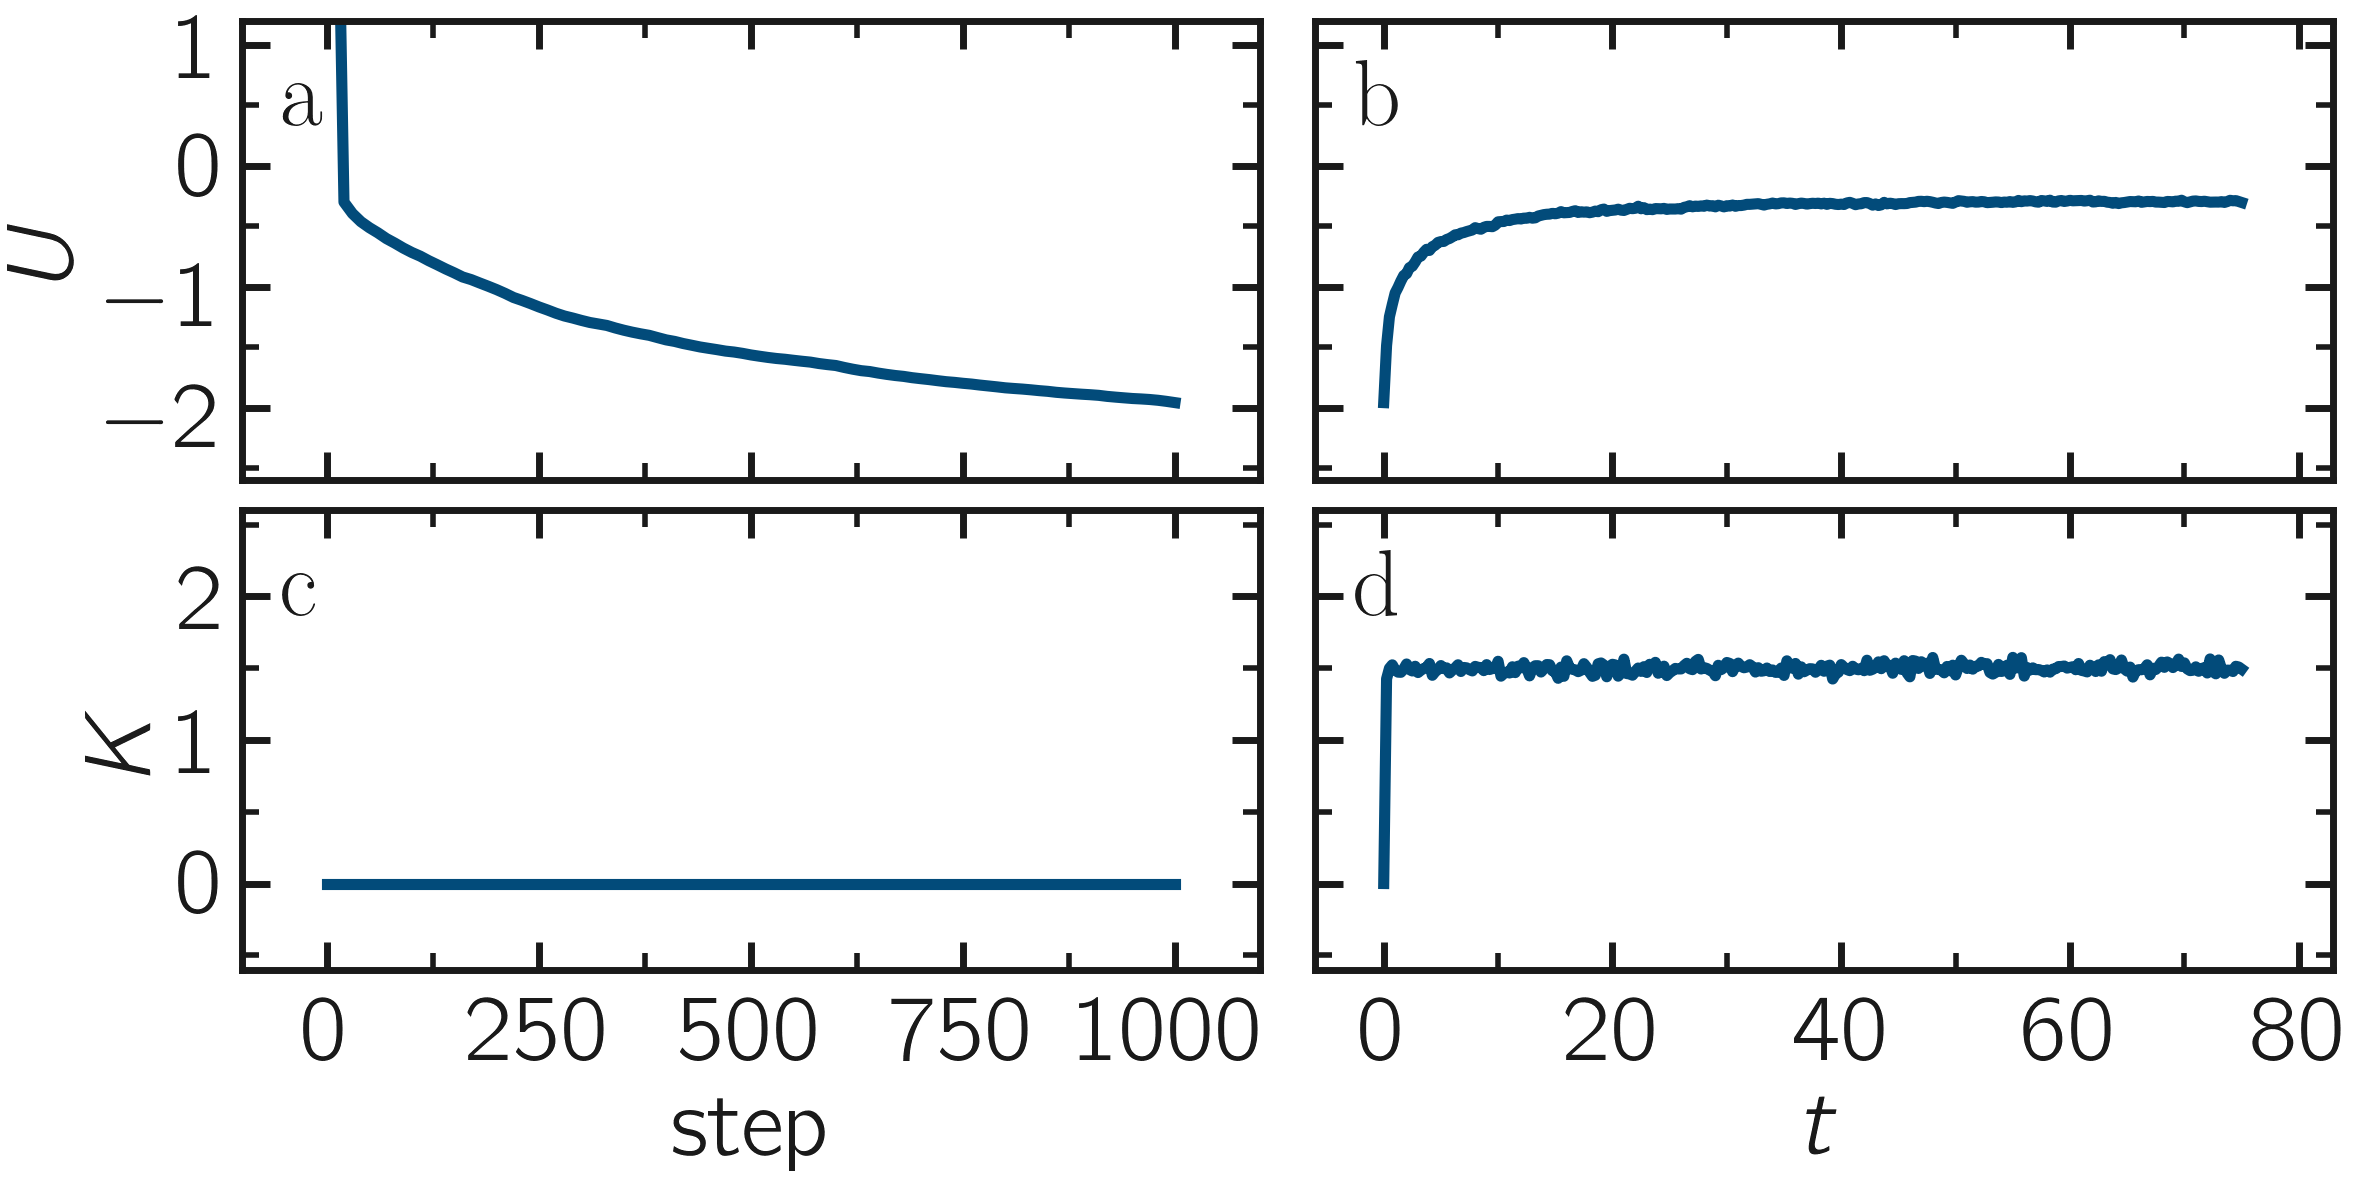
\includegraphics[width=\linewidth]{LJ-energy}
\caption{a) The potential energy ($p_\text{e}$) rapidly decreases during energy minimization (orange). Then, after the molecular dynamics simulation starts, $p_\text{e}$ increases until it reaches a plateau value of about -0.25 (blue). b) The kinetic energy ($k_\text{e}$) is equal to zero during energy minimization, then increases during molecular dynamics until it reaches a plateau value of about 1.5.}
\label{fig:evolution-energy}
\end{figure}

\paragraph{Trajectory visualization}

 To visualize the trajectories of the atoms, we first need to print the positions of the atoms in a file at a regular interval. Add the following command to the \textit{input.lammps} file, in the \textit{Visualization} section of \textit{PART B}:
 {\small \begin{verbatim}
dump mydmp all atom 100 dump.lammpstrj
\end{verbatim}}
Run the \textit{input.lammps} using LAMMPS again. The file named \textit{dump.lammpstrj} created by LAMMPS within \textit{my-first-input/} can be opened using VMD.

\subsubsection{Improving the script}

Let us improve the input script and perform slightly more advanced operations, such as imposing a specific initial
positions to the atoms, and restarting the simulation from a previously saved configuration. 

\paragraph{Control the initial atom positions}
\noindent Create a new folder next to \textit{my-first-input/}, and call it \textit{improved-input/}. Then, create a new input file within \textit{improved-input/} and call it \textit{input.min.lammps}. Similarly to what has been done previously, copy the following lines into \textit{input.min.lammps}:
{\small \begin{verbatim}
# 1) Initialization
units lj
dimension 3
atom_style atomic
pair_style lj/cut 2.5
boundary p p p
\end{verbatim}}
To create the atoms of types 1 and 2 in two separate regions, let us create three separate regions: A cubic region for the simulation box and two additional regions for placing the atoms:
{\small \begin{verbatim}
# 2) System definition
region simulation_box block -20 20 -20 20 -20 20
create_box 2 simulation_box
region cylinder_in cylinder z 0 0 10 INF INF side in
region cylinder_out cylinder z 0 0 10 INF INF side out
create_atoms 1 random 1000 341341 cylinder_out
create_atoms 2 random 150 127569 cylinder_in
\end{verbatim}}
The \textit{side in} and \textit{side out} keywords are used to define regions that are respectively inside and outside of the cylinder of radius 10. Then, copy similar lines as previously into \textit{input.min.lammps}:
{\small \begin{verbatim}
# 3) Simulation settings
mass 1 1
mass 2 1
pair_coeff 1 1 1.0 1.0
pair_coeff 2 2 0.5 3.0

# 4) Visualization
thermo 10
thermo_style custom step temp pe ke etotal press
dump mydmp all atom 10 dump.min.lammpstrj

# 5) Run
minimize 1.0e-4 1.0e-6 1000 10000
write_data minimized_coordinate.data
\end{verbatim}}
The main novelty, compared to the previous input script, is the \textit{write$\_$data} command. This command is used to print the final state of the simulation in a file named \textit{minimized$\_$coordinate.data}. Note that the \textit{write$\_$data} command is placed after the \textit{minimize} command. This \textit{.data} file will be used later to restart the simulation from the final state of the energy minimization step.

Run the \textit{input.min.lammps} script using LAMMPS. A new dump file named \textit{dump.min.lammpstrj} will appear in the folder, allowing you to visualize
the atom's trajectories during minimization. In addition, a file named \textit{minimized$\_$coordinate.data} will be created. If you open \textit{minimized$\_$coordinate.data} with a text editor, you can see that it contains all the information necessary to restart the simulation, such as the number of atoms and the box size, the \textit{masses}, the \textit{pair$\_$coeffs}.
The \textit{minimized$\_$coordinate.data} file also contains the final positions of the atoms within the \textit{Atoms} section.
The first five columns of the \textit{Atoms} section correspond (from left to right) to the atom indexes (from 1 to the total number of atoms, 1150), the atom types (1 or 2 here), and the atoms positions $x$, $y$, $z$. The last three columns are image flags that keep track of which atoms crossed the periodic boundary.

\paragraph{Restarting from a saved configuration}
Let us create a new input file and start a molecular dynamics simulation directly from the previously saved configuration. Within \textit{improved-input/}, create a new file named \textit{input.md.lammps} and copy the same lines as previously:
{\small \begin{verbatim}
# 1) Initialization
units lj
dimension 3
atom_style atomic
pair_style lj/cut 2.5
boundary p p p
\end{verbatim}}
Here, instead of creating a new region and adding atoms to it, we can simply import the previously saved configuration by adding the following command to \textit{input.md.lammps}:
{\small \begin{verbatim}
# 2) System definition
read_data minimized_coordinate.data
\end{verbatim}}
By visualizing the previously generated \textit{dump.min.lammpstrj} file, you may have noticed that some atoms have moved from one region to the other during minimization. To start the simulation from a clean slate, with only atoms of type 2 within the cylinder and atoms of type
1 outside the cylinder, let us delete the misplaced atoms by adding the following commands to \textit{input.md.lammps}:
{\small \begin{verbatim}
read_data minimized_coordinate.data
region cylinder_in cylinder z 0 0 10 INF INF &
    side in
region cylinder_out cylinder z 0 0 10 INF INF &
    side out
group group_type_1 type 1
group group_type_2 type 2
group group_region_in region cylinder_in
group group_region_out region cylinder_out
group group_type_1_in & 
    intersect group_type_1 group_region_in
group group_type_2_out &
    intersect group_type_2 group_region_out
delete_atoms group group_type_1_in
delete_atoms group group_type_2_out
\end{verbatim}}
The two first \textit{region} commands recreate the previously defined regions, which is necessary since regions are not saved by the \textit{write$\_$data} command. The first two \textit{group} commands create atom groups based on their types. The next two \textit{group} commands create atom groups based on their
positions at the beginning of the simulation, i.e. when the commands are being read by LAMMPS. The last two \textit{group} commands create atom groups based on the intersection between the previously defined groups. Finally, the two \textit{delete$\_$atoms} commands delete the atoms of type 1 that are located within the cylinder, as well as the atoms of type 2 that are located outside the cylinder, respectively. 
Add the following lines to \textit{input.md.lammps}. Note the absence of \textit{Simulation settings} section, because the settings are taken from the \textit{.data} file.
{\small \begin{verbatim}
# 4) Visualization
thermo 1000
dump mydmp all atom 1000 dump.md.lammpstrj
\end{verbatim}}
Let us extract the number of atoms of each type inside the cylinder as a function of time, by adding the following commands to \textit{input.md.lammps}:
{\small \begin{verbatim}
variable number_type1_in &
    equal count(group_type_1,cylinder_in)
variable number_type2_in & 
    equal count(group_type_2,cylinder_in)
fix myat1 all ave/time 10 200 2000 &
    v_number_type1_in &
    file output-population1vstime.dat
fix myat2 all ave/time 10 200 2000 &
    v_number_type2_in &
    file output-population2vstime.dat
\end{verbatim}}
The 2 \textit{variables} are used to count the number of atoms of a specific group in the \textit{cylinder$\_$in} region. The two \textit{fix ave/time} are calling the previously defined variables and are printing their values into text files. By using \textit{10 200 2000}, variables are evaluated every 10 steps, averaged 200 times, and printed in the \textit{.dat} files every 2000 steps.

\begin{figure}
\centering
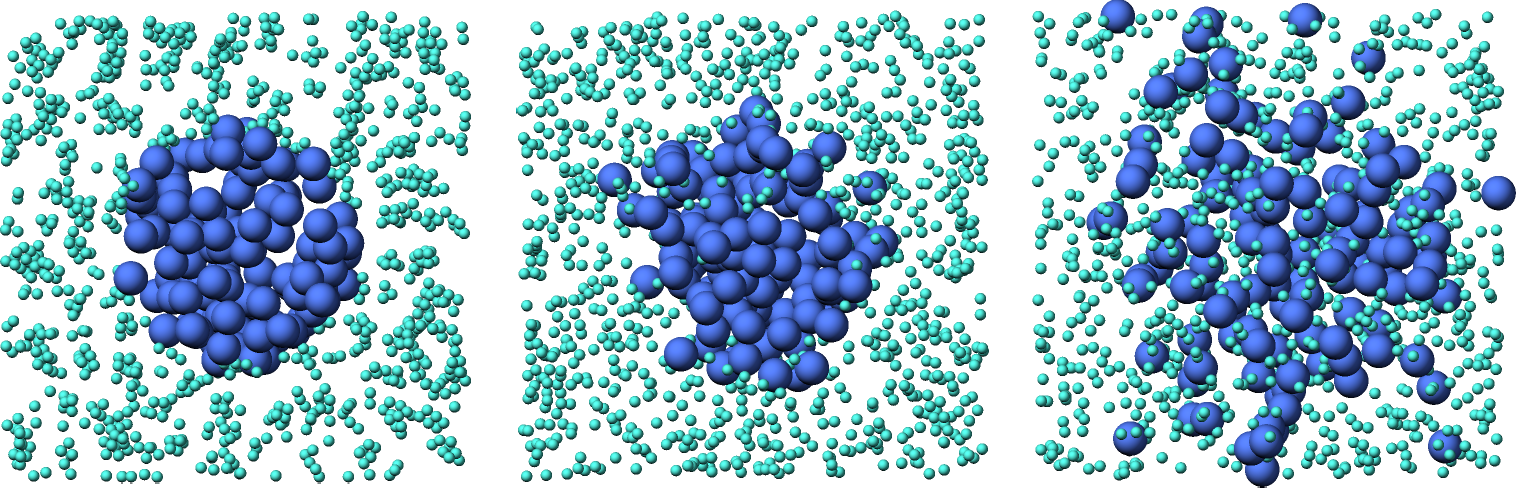
\includegraphics[width=\linewidth]{LJ-evolution}
\caption{Evolution of the system during mixing.}
\label{fig:evolution-population}
\end{figure}

Let us also extract the coordination number per atom between atoms of type 1 and 2, i.e. the average number of atoms of type 2 in the vicinity of the atoms of type 1. This coordination number will be used as an indicator of the degree of mixing of our binary mixture. Add the following lines into \textit{input.md.lammps}:
{\small \begin{verbatim}
compute coor12 group_type_1 coord/atom &
    cutoff 2.0 group group_type_2
compute sumcoor12 all reduce ave c_coor12
fix myat3 all ave/time 10 200 2000 &
    c_sumcoor12 file coordinationnumber12.dat
\end{verbatim}}
The \textit{compute ave} is used to average the per atom coordination number that is calculated by the \textit{coord/atom} compute. This averaging is necessary as \textit{coord/atom} returns an array where each value corresponds to a certain couple of atoms i-j. Such an array can't be printed by \textit{fix ave/time}. Finally, let us complete the script by adding the following lines to \textit{input.md.lammps}:
{\small \begin{verbatim}
# 5) Run
velocity all create 1.0 4928459 mom yes rot yes &
    dist gaussian
fix mynve all nve
fix mylgv all langevin 1.0 1.0 0.1 1530917 zero yes
timestep 0.005
run 300000
write_data mixed.data
\end{verbatim}}
There are a few differences from the previous simulation. First, the \textit{velocity create} command attributes an initial velocity to every atom.
The initial velocity is chosen so that the average initial temperature is equal to 1 (unitless). The additional keywords ensure that no linear momentum (\textit{mom yes}) and no angular momentum (\textit{rot yes}) are given to the system and that the generated velocities are distributed as a Gaussian. Another improvement is the \textit{zero yes} keyword in the Langevin thermostat, which ensures that the total random force is equal to zero.
Run \textit{input.md.lammps} using LAMMPS. Open the \textit{dump.md.lammpstrj} using VMD to observe the mixing of the two populations as the time evolves (Fig.\,\ref{fig:evolution-population}). The generated \textit{.dat} files indicate the number of atoms in each region as a function time (Fig.\,\ref{fig:mixing}\,a). In addition, as the mixing progresses, the calculated coordination number increases from about $0.01$ to $0.35$ (Fig.\,\ref{fig:mixing}\,b).

\begin{figure}
\centering
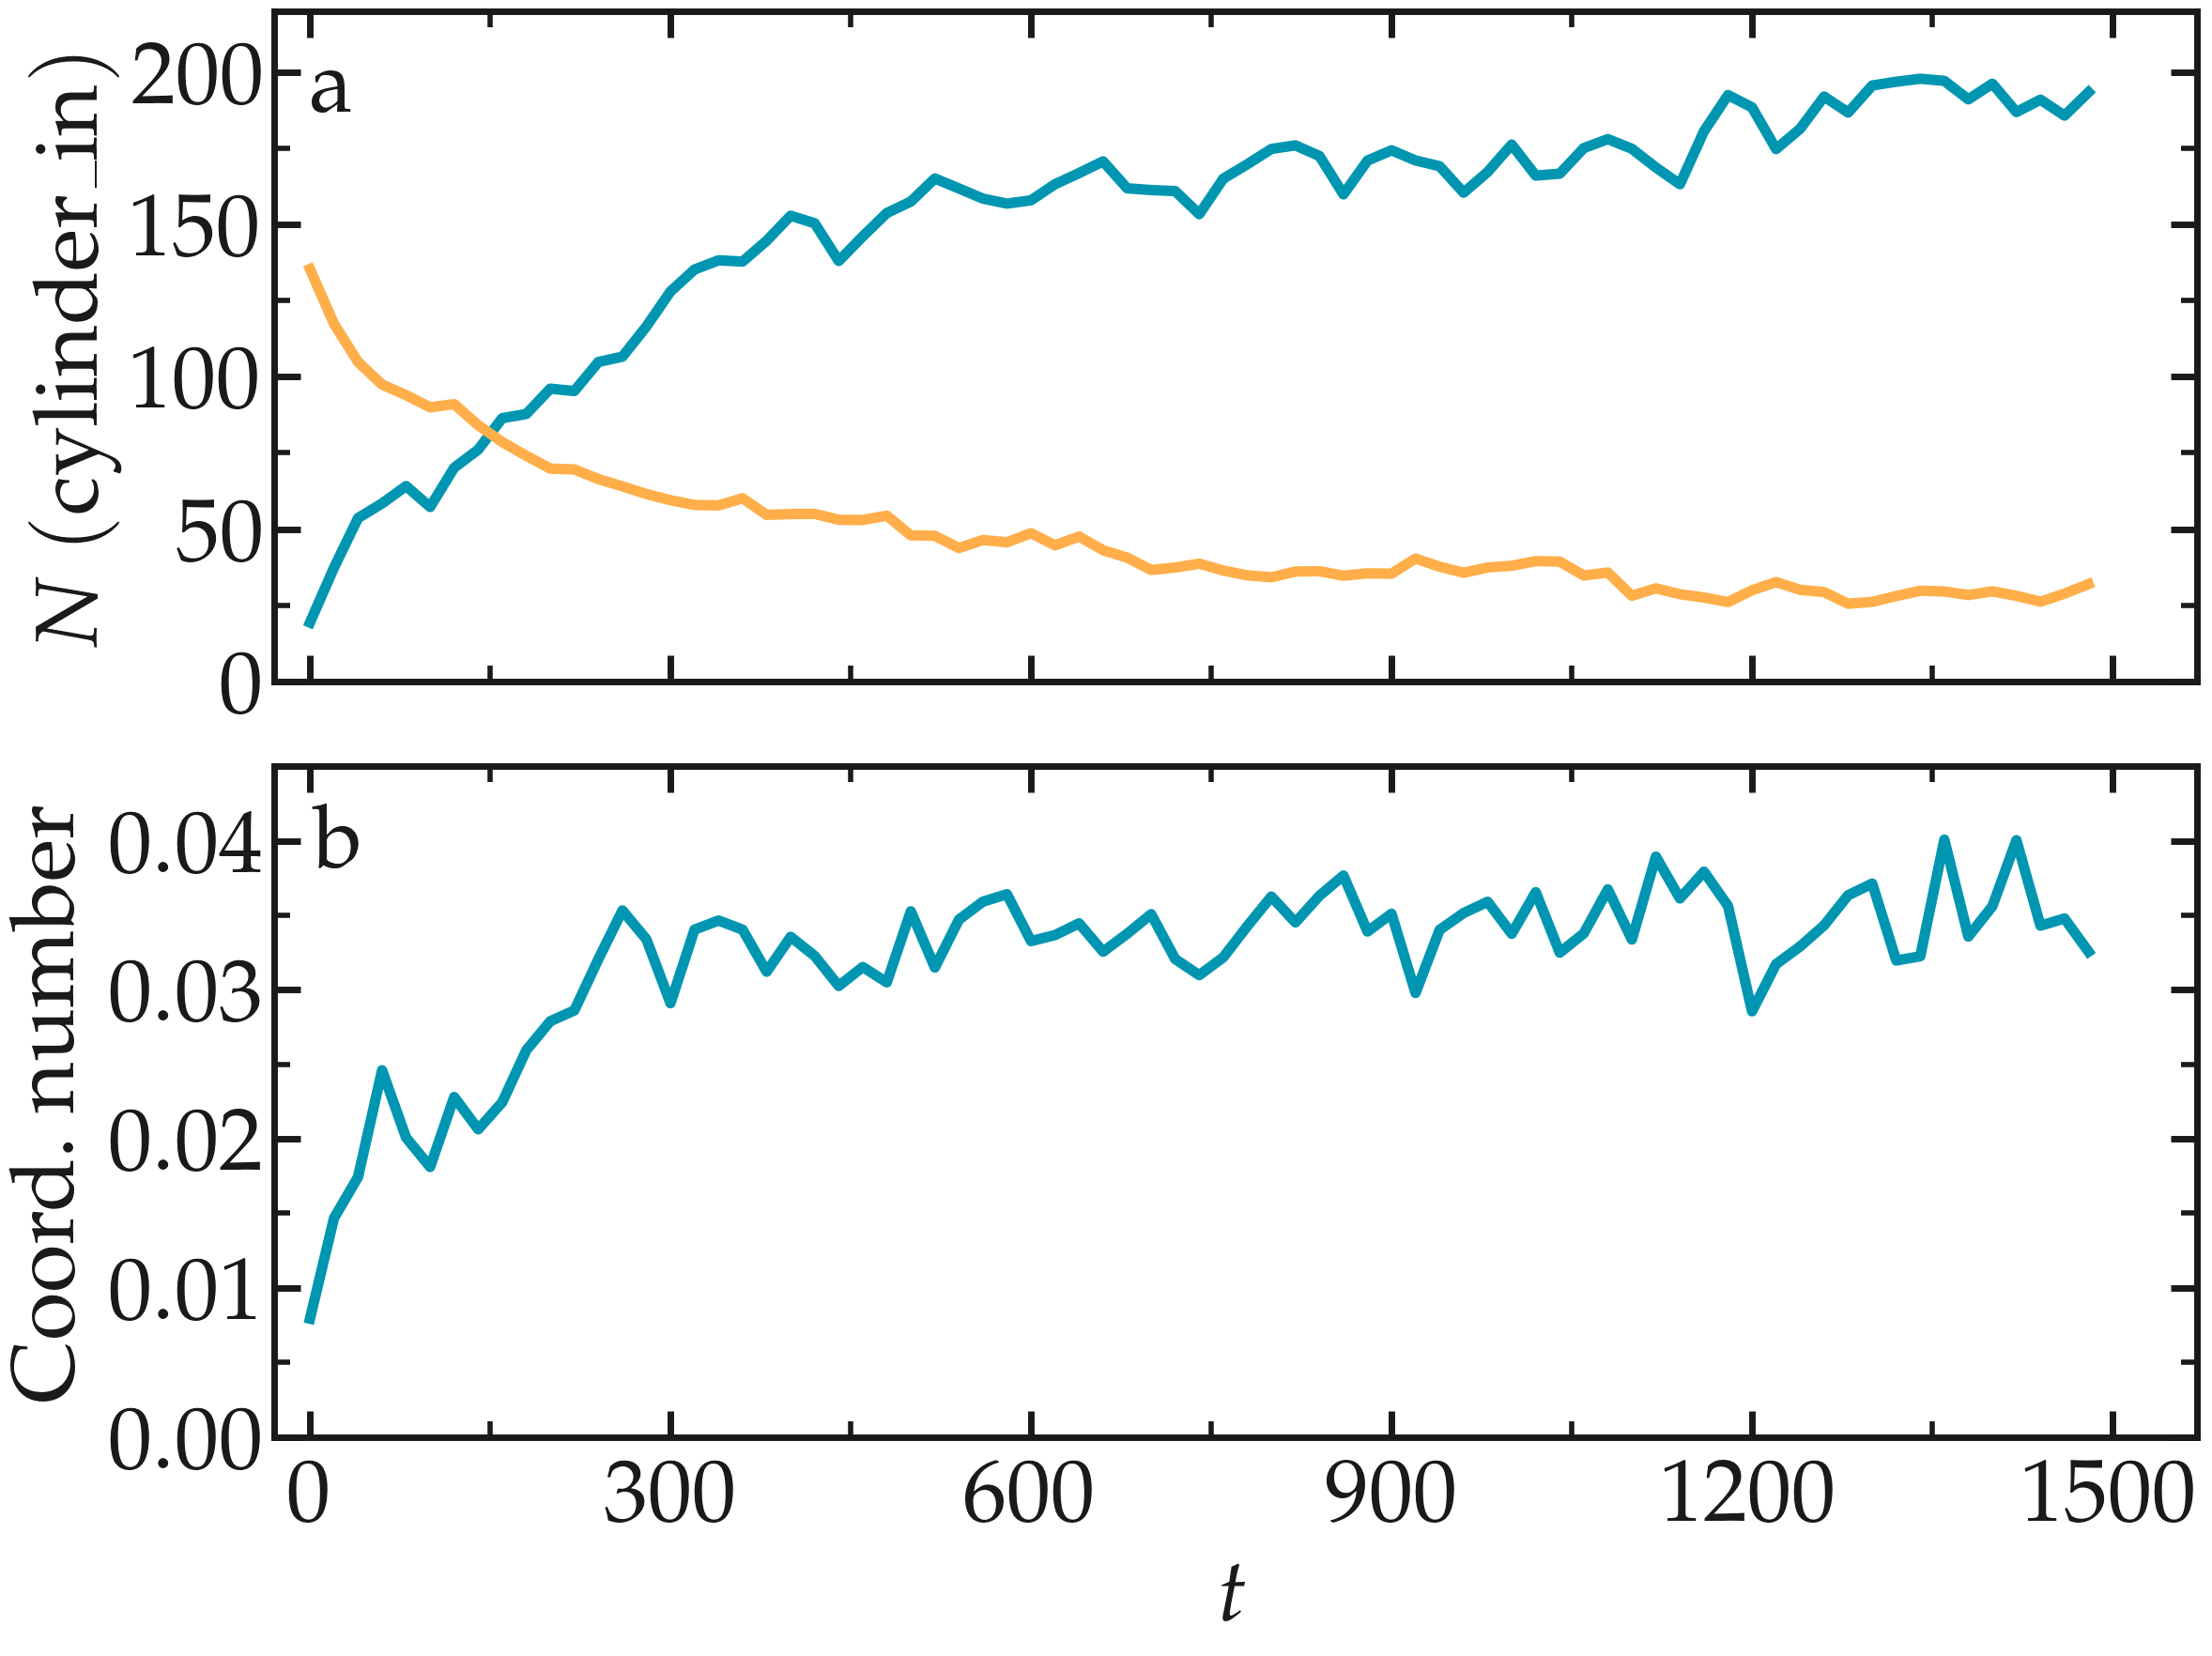
\includegraphics[width=\linewidth]{LJ-mixing}
\caption{a) Evolution of the number $N$ of atoms within the \textit{cylinder$\_$in} region as a function of the time $t$. b) Evolution of the coordination number.}
\label{fig:mixing}
\end{figure}

\subsection{Tutorial 2: Pulling on a carbon nanotube}
\label{carbon-nanotube-label}

\begin{figure}
{\centering
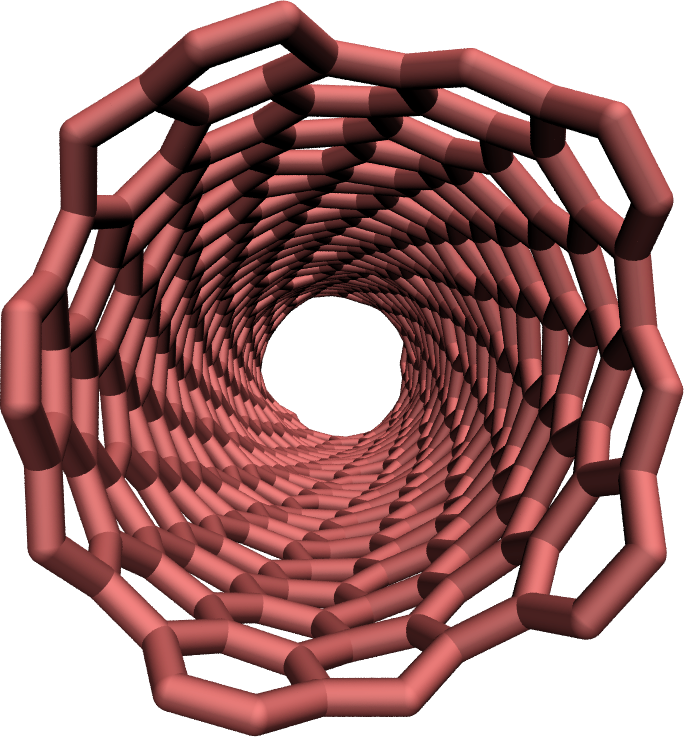
\includegraphics[width=0.55\linewidth]{CNT}
\caption{Snapshot of the carbon nanotube (CNT) made using VMD.}}
\label{fig:CNT}
\end{figure}

\vspace{0.25cm} \noindent The objective of this tutorial is to impose the deformation of a carbon nanotube (CNT) using LAMMPS. In this tutorial, a small carbon nanotube (CNT) is simulated within an empty box using LAMMPS (Fig.\,\ref{fig:CNT}). An external forcing is imposed on the CNT, and its deformation is measured with time. The difference between classical and reactive force fields
is illustrated through this tutorial. With a classical force field, the bonds between atoms are unbreakable. With the reactive force field (named AIREBO \cite{stuart2000reactive}), the breaking of the chemical bonds is possible when the imposed deformation is strong enough.

\subsubsection{Unbreakable bonds}
\noindent With most classical molecular dynamics force fields, the chemical bonds between the atoms are set at the start of the simulation. Regardless of the forces applied to the atoms during the simulations, the bonds remain intact. The bonds between neighbor atoms typically consist of springs with given equilibrium distances $r_0$ and a constant $k_b$: $U_b = k_b \left( r - r_0 \right)^2$.
Additionally, angular and dihedral constraints are usually applied to maintain the relative orientations of neighbor atoms. 

Download directly the CNT topology by clicking \href{https://lammpstutorials.github.io/lammpstutorials-inputs/level1/breaking-a-carbon-nanotube/unbreakable-bonds/cnt_molecular.data}{here}. It was created using VMD and TopoTools \cite{kohlmeyer2017topotools}, and contains information about the positions of the carbon atoms, as well as the
identity of the atoms that are linked by \textit{bonds}, \textit{angles}, \textit{dihedrals},
and \textit{impropers} constraints. Save the \textit{cnt$\_$molecular.data} file
in a folder named \textit{unbreakable-bonds/}.

\paragraph{The LAMMPS input}
Create a new text file within \textit{unbreakable-bonds/} and name it \textit{input.lammps}. Copy the following lines in it:
\begin{verbatim}
variable T equal 300

units real
atom_style molecular
boundary f f f
pair_style lj/cut 14

bond_style harmonic
angle_style harmonic
dihedral_style opls
improper_style harmonic

special_bonds lj 0.0 0.0 0.5

read_data cnt_molecular.data
\end{verbatim}
The chosen unit system is \textit{real} (therefore distances are in Ångstrom, time in femtosecond), the \textit{atom$\_$style} is molecular (therefore atoms are dots that can be bonded with each other), and the boundary conditions are fixed. The boundary conditions do not matter here, as the box boundaries were placed far from the CNT. 

Just like in the previous tutorial, \hyperref[lennard-jones-label]{Lennard Jones fluid}, the pair style is \textit{lj/cut} (i.e. a Lennard-Jones potential with a short-range cutoff) with parameter 14, which means that only the atoms closer than 14 Ångstroms from each other interact through a Lennard-Jones potential. The \textit{bond$\_$style}, \textit{angle$\_$style}, \textit{dihedral$\_$style}, and \textit{improper$\_$style} commands specify the different potentials used to restrain the relative positions of the atoms. For more details about the potentials used here, you can have a look at the LAMMPS website. The \textit{special$\_$bonds} command sets the weighting factors for the Lennard-Jones interaction between atoms directly connected by a bond, separated by two bonds, and separated by three bonds, respectively. The last command, \textit{read$\_$data}, imports the \textit{cnt$\_$molecular.data} file previously generated with VMD, which contains the information about the box size, atom positions, etc.

We need to specify the parameters of both bonded and non-bonded potentials. Here, the parameters are taken from the OPLS-AA (Optimised Potentials for Liquid Simulations-All-Atom) force field \cite{jorgensenDevelopmentTestingOPLS1996}. Create a new text file in the \textit{unbreakable-bonds/} folder and name it \textit{parm.lammps}. Copy the following lines in it:
\begin{verbatim}
pair_coeff 1 1 0.066 3.4
bond_coeff 1 469 1.4
angle_coeff 1 63 120
dihedral_coeff 1 0 7.25 0 0
improper_coeff 1 5 180
\end{verbatim}
The \textit{pair$\_$coeff} command sets the parameters for the non-bonded Lennard-Jones interaction $\epsilon_{11} = 0.066 \, \text{kcal/mol}$ and $\sigma_{11} = 3.4 \, \text{Å}$ for the only type of atom of the simulation; the carbon atom of type 1.  The \textit{bond$\_$coeff} provides the equilibrium distance $r_0= 1.4 \, \text{Å}$ as well as the spring constant $k_b = 469 \, \text{kcal/mol/Å}^2$ for the harmonic potential imposed between two neighboring carbon atoms, where the potential is $U_b = k_b ( r - r_0)^2$. The
\textit{angle$\_$coeff} gives the equilibrium angle $\theta_0$ and constant for the potential between three neighbor atoms :
$U_\theta = k_\theta ( \theta - \theta_0)^2$. The \textit{dihedral$\_$coeff} and \textit{improper$\_$coeff} gives the potential for the constraints between 4 atoms. The file \textit{parm.lammps} is included in the simulation by adding the following line to the \textit{input.lammps} file:
\begin{verbatim}
include parm.lammps
\end{verbatim}

\paragraph{Prepare initial state}
Before starting the molecular dynamics simulation, let us make sure that we start from a clean initial state
by recentering the CNT at the origin (0, 0, 0). In addition, let us make sure that the box boundaries are symmetric with respect to (0, 0, 0), which is not initially the case, as seen in \textit{cnt$\_$molecular.data}:
\begin{verbatim}
-40.000000 40.000000  xlo xhi
-40.000000 40.000000  ylo yhi
-12.130411 67.869589  zlo zhi
\end{verbatim}
Let us recenter the CNT by adding the following lines to \textit{input.lammps}:
\begin{verbatim}
group carbon_atoms type 1
variable carbon_xcm equal -1*xcm(carbon_atoms,x)
variable carbon_ycm equal -1*xcm(carbon_atoms,y)
variable carbon_zcm equal -1*xcm(carbon_atoms,z)
displace_atoms carbon_atoms &
    move ${carbon_xcm} ${carbon_ycm} ${carbon_zcm}
\end{verbatim}
The first command includes all the atoms of type 1 (i.e. all the atoms here) in a group named \textit{carbon$\_$atoms}. 
The 3 variables, \textit{carbon$\_$xcm}, \textit{carbon$\_$ycm}, and \textit{carbon$\_$zcm} are used to measure
the current position of the group \textit{carbon$\_$atoms} along all 3 directions, respectively. Then, the \textit{displace$\_$atoms} 
command move the group \textit{carbon$\_$atoms}, ensuring that its center of mass is located at the origin (0, 0, 0).
Let us also change the box boundaries by adding the following line to \textit{input.lammps}:
\begin{verbatim}
change_box all x final -40 40 y final -40 40 &
    z final -40 40
\end{verbatim}
Such a cleaner and more symmetrical initial state can simplify future data analysis, but won't make any difference to the molecular dynamics.

A displacement will be imposed on the edges of the CNT. To do so, let us isolate the atoms from the two edges and place them into groups named \textit{rtop} and \textit{rbot}, respectively. Add the following lines to \textit{input.lammps}:
\begin{verbatim}
variable zmax equal bound(carbon_atoms,zmax)-0.5
variable zmin equal bound(carbon_atoms,zmin)+0.5
region rtop block INF INF INF INF ${zmax} INF
region rbot block INF INF INF INF INF ${zmin}
region rmid block INF INF INF INF ${zmin} ${zmax}
\end{verbatim}

\noindent The variable $z_\mathrm{max}$ corresponds to the coordinate of the last atoms along $z$ minus 0.5 Ångstroms, and $z_\mathrm{min}$ to the coordinate of the first atoms along $z$ plus 0.5 Ångstroms. Then, 3 regions are defined, and correspond respectively to: $z < z_\mathrm{min}$, (bottom) $z_\mathrm{min} > z > z_\mathrm{max}$ (middle), and $z > z_\mathrm{max}$ (top). Finally, let us define 3 groups of atoms corresponding to the atoms located in each of the 3 regions, respectively, by adding to \textit{input.lammps}:
\begin{verbatim}
group carbon_top region rtop
group carbon_bot region rbot
group carbon_mid region rmid
\end{verbatim}
The atoms of the edges as selected within the \textit{carbon$\_$top} and \textit{carbon$\_$bot} groups can be represented with a different color.

\begin{figure}
\centering
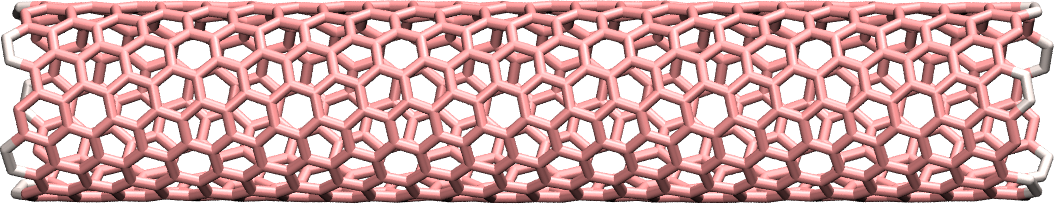
\includegraphics[width=\linewidth]{CNT-underformed}
\caption{CNT with atoms from the \textit{carbon$\_$top} and the \textit{carbon$\_$bot} groups are represented with a different color.}
\label{fig:CNT-underformed}
\end{figure}

When running a simulation, the number of atoms in each group is printed in the terminal (and in the \textit{log.lammps} file). Always make sure that the number of atoms in each group corresponds to what is expected, just like here:
\begin{verbatim}
10 atoms in group carbon_top
10 atoms in group carbon_bot
680 atoms in group carbon_mid
\end{verbatim}
Finally, let us randomly delete some of the carbon atoms. In order to avoid deleting atoms that are too close to the edges, let us define a new region name \textit{rdel} that starts $2\,Å$ from the CNT edges.
\begin{verbatim}
variable zmax_del equal ${zmax}-2
variable zmin_del equal ${zmin}+2
region rdel block INF INF INF INF &
    ${zmin_del} ${zmax_del}
group rdel region rdel
delete_atoms random fraction 0.02 no rdel &
    NULL 482793 bond yes
\end{verbatim}
The \textit{delete$\_$atoms} command randomly deletes $2\,\%$ of the atoms from the \textit{rdel} group (i.e. about 10 atoms) (Fig.\,\ref{fig:CNT-underformed-deleted}).

\begin{figure}
\centering
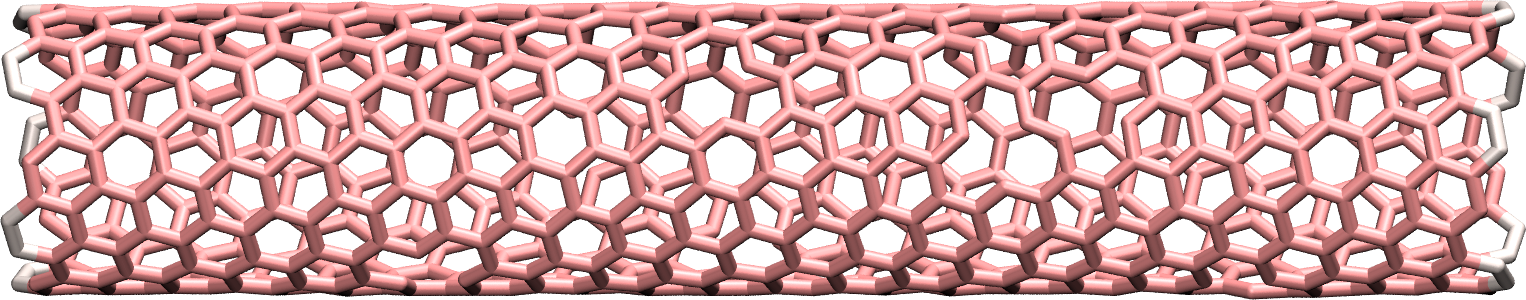
\includegraphics[width=\linewidth]{CNT-underformed-deleted}
\caption{CNT with \textit{10} randomly deleted atoms.}
\label{fig:CNT-underformed-deleted}
\end{figure}

\paragraph{The molecular dynamics}
Let us specify the thermalization and the dynamics of the system. Add the following lines to \textit{input.lammps}:
\begin{verbatim}
reset_atoms id sort yes
velocity carbon_mid create ${T} 48455 mom yes &
    rot yes
fix mynve all nve
compute Tmid carbon_mid temp
fix myber carbon_mid temp/berendsen ${T} ${T} 100
fix_modify myber temp Tmid
\end{verbatim}
Re-setting the atom ids is necessary before using the \textit{velocity} command, this is done by the \textit{reset$\_$atoms} command.
The \textit{velocity} command gives initial velocities to the atoms of the middle group \textit{carbon$\_$mid}, ensuring an initial temperature of 300 K for these atoms with no overall translational momentum, \textit{mom yes}, nor rotational momentum, \textit{rot yes}.
The \textit{fix nve} is applied to all atoms so that all atom positions are recalculated at every step, and a \textit{Berendsen} thermostat is applied to the atoms of the group \textit{carbon$\_$mid} only \cite{berendsen1984molecular}. The \textit{fix$\_$modify myber} ensures that the \textit{fix Berendsen} uses the temperature of the group \textit{carbon$\_$mid} as an input, instead of the temperature of the whole system. This is necessary to make sure that the frozen edges won't bias the temperature. Note that the atoms
of the edges do not need a thermostat because their motion will be restrained, see below.

To restrain the motion of the atoms at the edges, let us add the following commands to \textit{input.lammps}:
\begin{verbatim}
fix mysf1 carbon_top setforce 0 0 0
fix mysf2 carbon_bot setforce 0 0 0
velocity carbon_top set 0 0 0
velocity carbon_bot set 0 0 0
\end{verbatim}
The two \textit{setforce} commands cancel the forces applied on the atoms of the two edges, respectively. The cancellation of the forces
is done at every step, and along all 3 directions of space, $x$, $y$, and $z$, due to the use of \textit{0 0 0}. The two \textit{velocity} commands set the initial velocities along $x$, $y$, and $z$ to 0 for the atoms of \textit{carbon$\_$top} and \textit{carbon$\_$bot}, respectively. As a consequence of these last four commands, the atoms of the edges will remain immobile during the simulation (or at least they would if no other command was applied to them). The \textit{velocity set} commands impose the velocity of a group of atoms at the start of a run, but does not enforce the velocity during the entire simulation. When \textit{velocity set} is used in combination with \textit{setforce 0 0 0}, as is the case here, the atoms won't feel any force during the entire simulation. According to the Newton equation, no force means no acceleration, meaning that the initial velocity will persist during the entire simulation, thus producing a constant velocity motion.

\paragraph{Data extraction}
Next, in order to measure the strain and stress suffered by the CNT, let us extract the distance $L$ between the two edges as well as the force applied on the edges.
\begin{verbatim}
variable L equal xcm(carbon_top,z)-xcm(carbon_bot,z)
fix at1 all ave/time 10 10 100 v_L &
    file output_cnt_length.dat
fix at2 all ave/time 10 10 100 f_mysf1[1] &
    f_mysf2[1] file output_edge_force.dat
\end{verbatim}
\noindent Let us also add a command to print the atom coordinates in a \textit{lammpstrj} file every 1000 steps.
\begin{verbatim}
dump mydmp all atom 1000 dump.lammpstrj
\end{verbatim}
\noindent Finally, let us check the temperature of the non-frozen group over time by printing it using a \textit{fix ave/time} command:
\begin{verbatim}
fix at3 all ave/time 10 10 100 c_Tmid &
    file output_temperature_middle_group.dat
\end{verbatim}

Let us run a small equilibration step to bring the system to the required temperature before applying any deformation:
\begin{verbatim}
thermo 100
thermo_modify temp Tmid

timestep 1.0
run 5000
\end{verbatim}
With the \textit{thermo$\_$modify} command, we specify to LAMMPS that we want the temperature $T_\mathrm{mid}$ to be printed in
the terminal, not the temperature of the entire system (because of the frozen edges, the temperature of the entire system is not relevant).
Let us impose a constant velocity deformation on the CNT by combining the \textit{velocity set} command with previously defined \textit{fix setforce}. Add the following lines in the \textit{input.lammps} file, right after the last \textit{run 5000} command:
\begin{verbatim}
velocity carbon_top set 0 0 0.0005
velocity carbon_bot set 0 0 -0.0005
run 10000
\end{verbatim}
\noindent The chosen velocity for the deformation is $100\,\text{m/s}$, or $0.001\,\text{Å/fs}$.

\begin{figure}
\centering
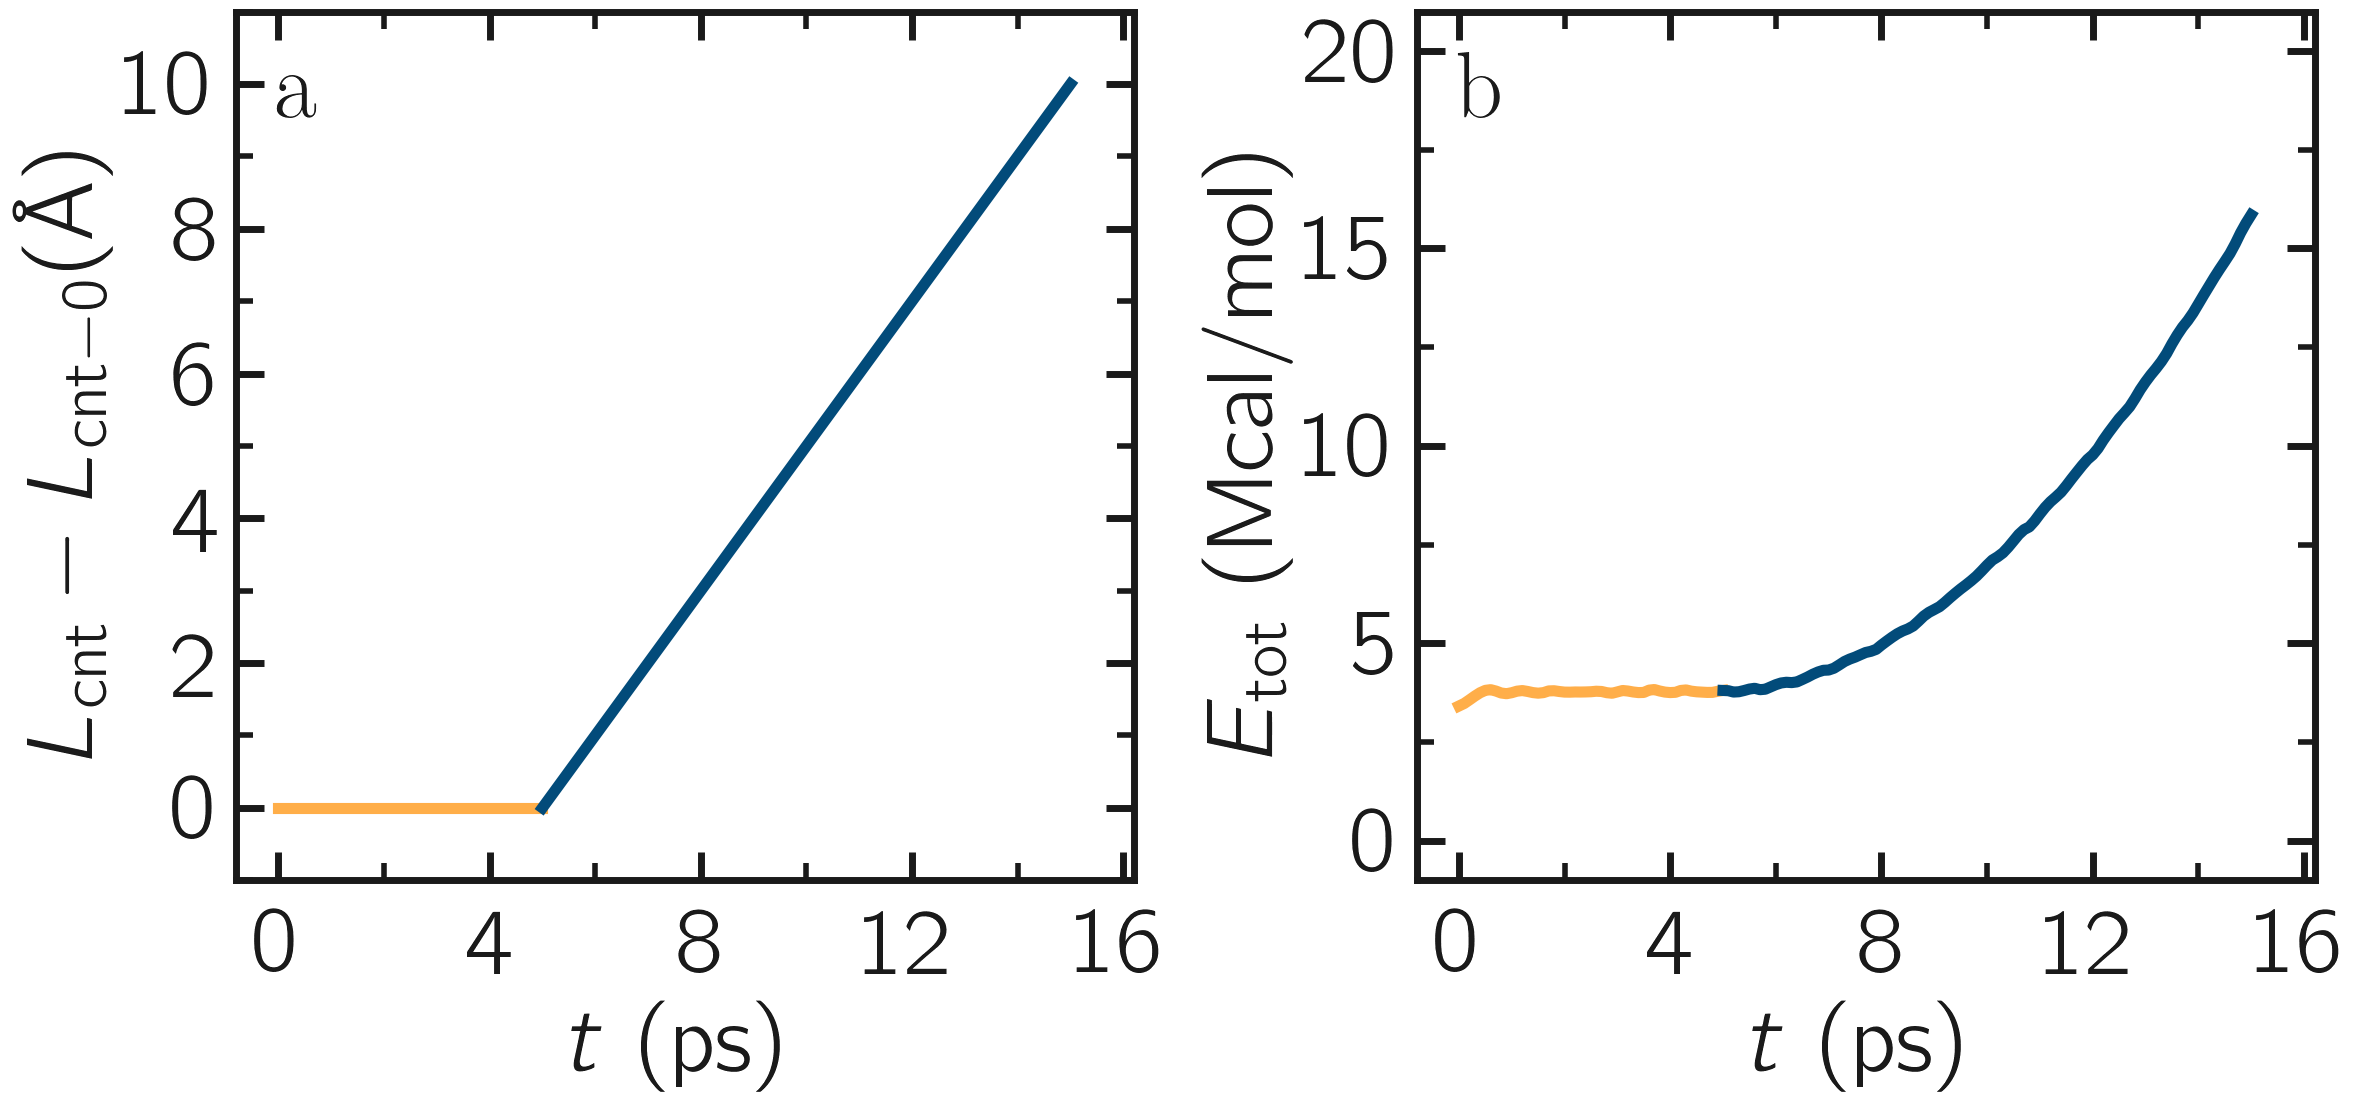
\includegraphics[width=\linewidth]{CNT-lenght-unbreakable}
\caption{Evolution of the length of the CNT with time. The CNT starts deforming at $t = 5\,\text{ps}$.}
\label{fig:CNT-unbreakable-lenght}
\end{figure}

The energy, which can be accessed from the log file, shows a non-linear increase with time once the deformation starts, which is expected from the typical dependency of bond energy with bond distance $U_b = k_b \left( r - r_0 \right)^2$ (Fig.\,\ref{fig:CNT-unbreakable-energy}).
As always, is it important to ensure that the simulation behaves as expected by opening the \textit{dump.lammpstrj} file with VMD (Fig.\,\ref{fig:CNT-deformed-unbreakable}).

\begin{figure}
\centering
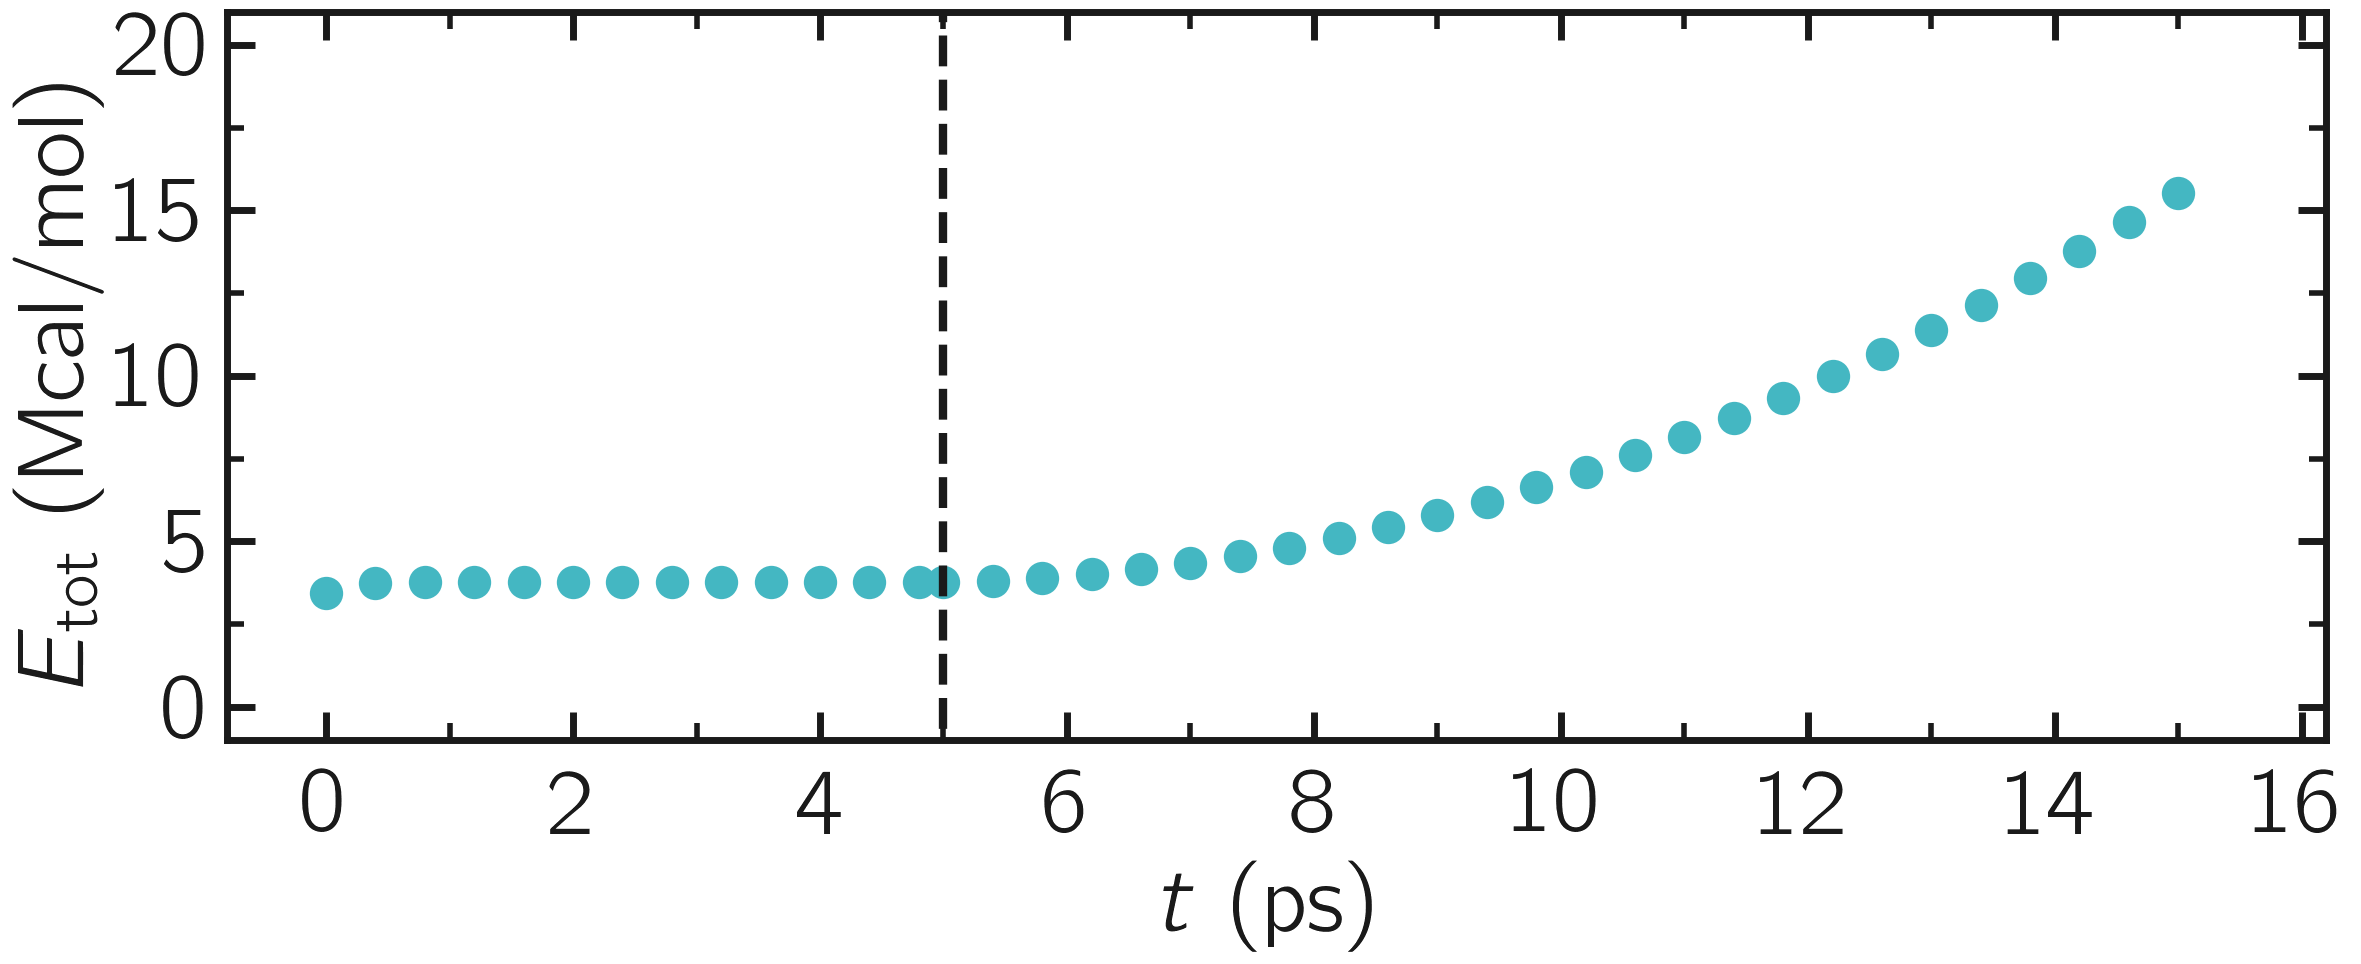
\includegraphics[width=\linewidth]{CNT-energy-unbreakable}
\caption{Evolution of the total energy of the system with time. The CNT starts deforming at $t = 5\,\text{ps}$.}
\label{fig:CNT-unbreakable-energy}
\end{figure}

\begin{figure}
\centering
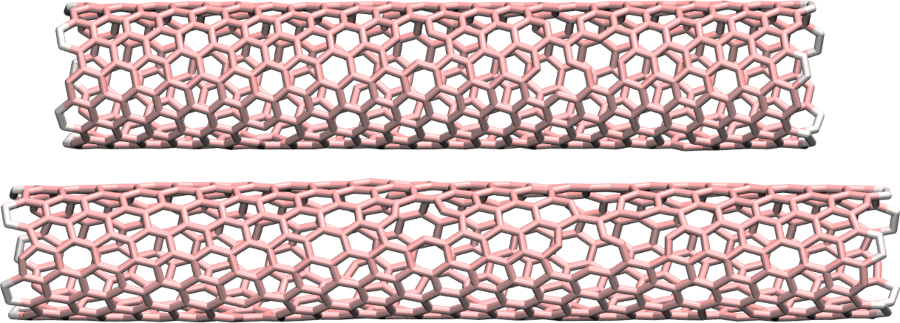
\includegraphics[width=\linewidth]{CNT-deformed-unbreakable}
\caption{CNT before (top) and after (bottom) deformation.}
\label{fig:CNT-deformed-unbreakable}
\end{figure}

\subsubsection{Breakable bonds}
When using a classical force field, as we just did, the bonds between atoms are non-breakable. Let us perform a similar simulation, 
but this time using a reactive force field instead, allowing for the bonds to break if the applied deformation is large enough.

\paragraph{Input file initialization}
\noindent Create a second folder named \textit{breakable-bonds/} next to \textit{unbreakable-bonds/}, and create a new input file in it called \textit{input.lammps}. Type into input.lammps:
\begin{verbatim}
# Initialisation
variable T equal 300

units metal
atom_style atomic
boundary p p p
pair_style airebo 2.5 1 1
\end{verbatim}
The first difference with the previous part is the unit system, here \textit{metal} instead of \textit{real}, a choice that is imposed by the AIREBO force field. A second difference is the use of the \textit{atom$\_$style atomic} instead of \textit{molecular}, single no explicit bond information is required with AIREBO.

\paragraph{Adapt the topology file}
Since \textit{bond}, \textit{angle}, and \textit{dihedral} do not need to be explicitly set when using AIREBO, some small changes need to be made to the previously generated \textit{.data} file. Duplicate the previous file \textit{cnt$\_$molecular.data}, name the copy \textit{cnt$\_$atom.data}, place it within \textit{breakable-bonds/}. Then, remove all bond, angle, and dihedral information from \textit{cnt$\_$atom.data}. Also, remove the second column of the \textit{Atoms} table, so that the \textit{cnt$\_$atom.data} looks like the following: 
\begin{verbatim}
700 atoms
1 atom types
-40.000000 40.000000  xlo xhi
-40.000000 40.000000  ylo yhi
-12.130411 67.869589  zlo zhi

Masses

1 12.010700 # CA

Atoms # atomic

1 1 5.162323 0.464617 8.843235 # CA CNT
2 1 4.852682 1.821242 9.111212 # CA CNT
(...)
\end{verbatim}
In addition, remove the \textit{Bonds} table that is placed right after the \textit{Atoms} table (near line 743), as well as the \textit{Angles}, \textit{Dihedrals}, and \textit{Impropers} tables. The last lines of the file should look like this:
\begin{verbatim}
(...)
697 1 4.669892 -2.248901 45.824036 # CA CNT
698 1 5.099893 -0.925494 46.092010 # CA CNT
699 1 5.162323 -0.464617 47.431896 # CA CNT
700 1 5.099893 0.925494 47.699871 # CA CNT
\end{verbatim}

\paragraph{Use of AIREBO potential}
Then, let us import the LAMMPS data file, and set the pair coefficients by adding the following lines to \textit{input.lammps}
\begin{verbatim}
# System definition
read_data cnt_atom.data
pair_coeff * * CH.airebo C
\end{verbatim}
Here, there is one single atom type. We impose this type to be carbon by using the letter \textit{C}. The \textit{CH.airebo} file can be
downloaded by clicking \href{https://lammpstutorials.github.io/lammpstutorials-inputs/level1/breaking-a-carbon-nanotube/breakable-bonds/CH.airebo}{here}, and must be placed within the \textit{breakable-bonds/} folder. The rest of the \textit{input.lammps} is very similar to the previous one:

\begin{verbatim}
change_box all x final -40 40 y final -40 40 &
    z final -60 60

group carbon_atoms type 1
variable carbon_xcm equal -1*xcm(carbon_atoms,x)
variable carbon_ycm equal -1*xcm(carbon_atoms,y)
variable carbon_zcm equal -1*xcm(carbon_atoms,z)
displace_atoms carbon_atoms move ${carbon_xcm} &
    ${carbon_ycm} ${carbon_zcm}

variable zmax equal bound(carbon_atoms,zmax)-0.5
variable zmin equal bound(carbon_atoms,zmin)+0.5
region rtop block INF INF INF INF ${zmax} INF
region rbot block INF INF INF INF INF ${zmin}
region rmid block INF INF INF INF ${zmin} ${zmax}

group carbon_top region rtop
group carbon_bot region rbot
group carbon_mid region rmid

variable zmax_del equal ${zmax}-2
variable zmin_del equal ${zmin}+2
region rdel block INF INF INF INF &
    ${zmin_del} ${zmax_del}
group rdel region rdel
delete_atoms random fraction 0.02 no rdel &
    NULL 482793

reset_atoms id sort yes
velocity carbon_mid create ${T} 48455 mom yes &
    rot yes
fix mynve all nve
compute Tmid carbon_mid temp
fix myber carbon_mid temp/berendsen ${T} ${T} 0.1
fix_modify myber temp Tmid
\end{verbatim}
Note that a large distance of 120 Ångstroms was used for the box size along the \textit{z} axis, to allow for larger deformation. In addition, the \textit{change$\_$box} command was placed before the \textit{displace$\_$atoms} to avoid issue with the CNT crossing the edge of the box.

\paragraph{Start the simulation}
Here, let us impose a constant velocity deformation using the atoms of one edge, while maintaining the other edge fix. Do to so,
one needs to cancel the forces (thus the acceleration) on the atoms of the edges using the \textit{setforce} command and set the value of the velocity along the \textit{z} direction. First, as an equilibration step, let us set the velocity to 0 for the atoms of both edges. Let us fully constrain the edges. Add the following lines to LAMMPS:
\begin{verbatim}
fix mysf1 carbon_bot setforce 0 0 0
fix mysf2 carbon_top setforce 0 0 0
velocity carbon_bot set 0 0 0
velocity carbon_top set 0 0 0

variable L equal &
    xcm(carbon_top,z)-xcm(carbon_bot,z)
fix at1 all ave/time 10 10 100 v_L file &
    output_cnt_length.dat
fix at2 all ave/time 10 10 100 f_mysf1[1] &
    f_mysf2[1] file output_edge_force.dat

dump mydmp all atom 1000 dump.lammpstrj

thermo 100
thermo_modify temp Tmid

timestep 0.0005
run 5000
\end{verbatim}
Note the relatively small timestep of $0.0005\,\text{ps}$ used. A reactive force field usually requires a smaller timestep than a classical one. When running \textit{input.lammps} with LAMMPS, you can see that the temperature deviates from the target temperature of $300\,\text{K}$ at the start of the equilibration, but that after a few steps, it reaches the target value.

\paragraph{Launch the deformation}
After equilibration, let us set the velocity to 15 m/s and run for a longer duration than previously. Add the following lines into \textit{input.lammps}:
\begin{verbatim}
# 0.15 A/ps = 15 m/s
velocity carbon_top set 0 0 0.15
run 280000
\end{verbatim}
The CNT should break around step 250000. If not, use a longer run. When looking at the \textit{lammpstrj} file using VMD, you will see the bonds breaking (Fig.\,\ref{fig:CNT-breakable-energy}). From VMD, use the \textit{DynamicBonds} representation to properly visualize the bond breaking.

\begin{figure}
\centering
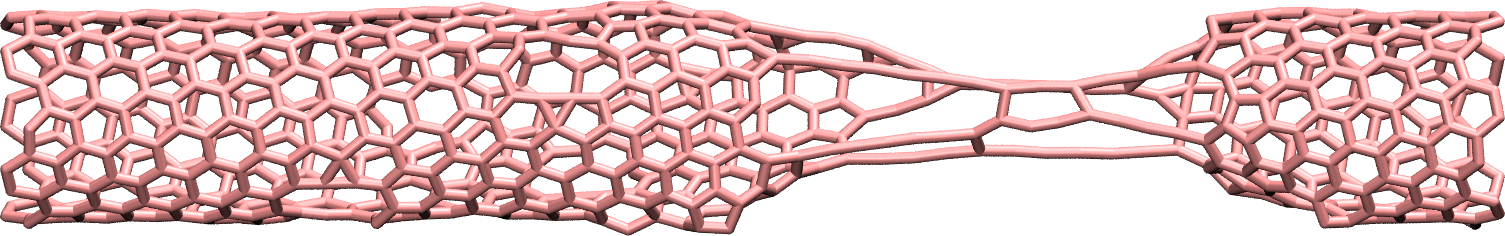
\includegraphics[width=\linewidth]{CNT-deformed-breakable}
\caption{CNT with broken bonds.}
\label{fig:CNT-deformed-breakable}
\end{figure}

Looking at the evolution of energy again, one can see that the energy in increasing with the deformation, before completely relaxing when the CNT finally breaks (Fig.\,\ref{fig:CNT-breakable-energy}).

\begin{figure}
\centering
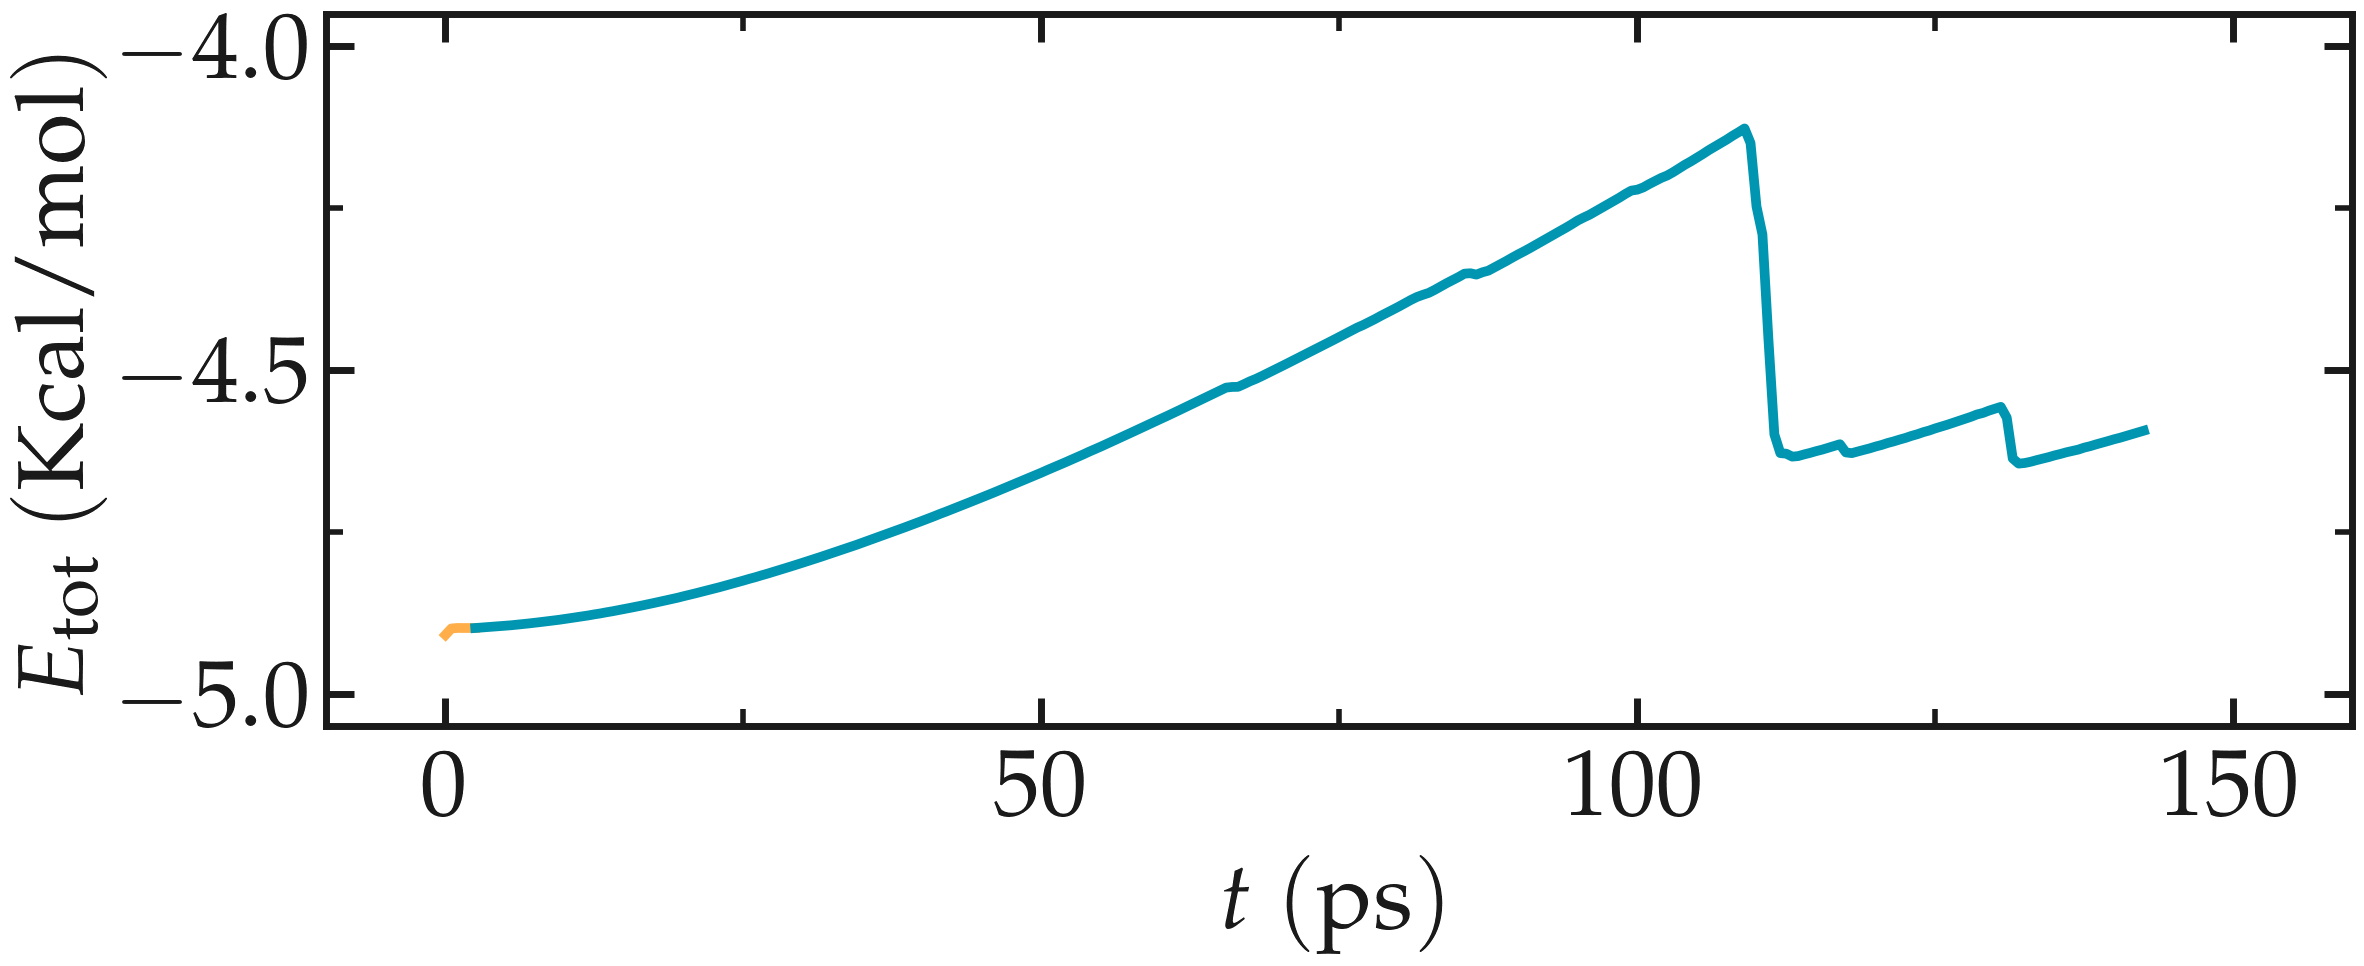
\includegraphics[width=\linewidth]{CNT-energy-breakable}
\caption{Evolution of the total energy of the system with time.}
\label{fig:CNT-breakable-energy}
\end{figure}

\subsection{Tutorial 3: Polymer in water}
\label{all-atoms-label}

\begin{figure}
\centering
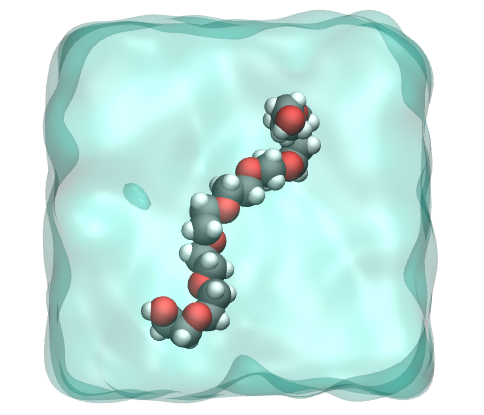
\includegraphics[width=0.55\linewidth]{PEG}
\caption{Snapshot of the PEG polymer molecule in water. Water molecules are represented as a transparent continuum field for clarity.}
\label{fig:PEG}
\end{figure}

The goal of this tutorial is to use LAMMPS and solvate a small hydrophilic polymer (PEG - PolyEthylene Glycol) in a reservoir of water (Fig.\,\ref{fig:PEG}). An all-atom description is used for both PEG (GROMOS 54A7 force field \cite{schmid2011definition}) and water (SPC/Fw model \cite{wu2006flexible}) and the long range Coulomb interactions are solved using the PPPM solver \cite{luty1996calculating}. Once the water reservoir is properly equilibrated at the desired temperature and pressure, the polymer molecule is added and a constant stretching force is applied to both ends of the polymer. The evolution of the polymer length is measured as a function of time. This tutorial was inspired by a publication by Liese and coworkers, in which molecular dynamics simulations are compared with force spectroscopy experiments \cite{liese2017hydration}.

\subsubsection{Preparing the water reservoir}

In this tutorial, the water reservoir is first prepared in the absence of polymer. A rectangular box of water is created and
equilibrated at ambient temperature and ambient pressure. The SPC/Fw water model is used \cite{wu2006flexible}, which is
a flexible variant of the rigid SPC (simple point charge) model \cite{berendsen1981interaction}. Create a folder named \textit{pureH2O/}. Inside this folder, create an empty text file named \textit{input.lammps}. Copy the following lines in it:
\begin{verbatim}
units real
atom_style full
bond_style harmonic
angle_style harmonic
dihedral_style harmonic
pair_style lj/cut/coul/long 12
kspace_style pppm 1e-5
special_bonds lj 0.0 0.0 0.5 &
    coul 0.0 0.0 1.0 angle yes
\end{verbatim}
With the unit style \textit{real}, masses are in grams per mole, distances in Ångstroms, time in femtoseconds, energies
in Kcal/mole. With the \textit{atom$\_$style full}, each atom is a dot with a mass and a charge that can be linked by bonds, angles, dihedrals and/or impropers. The \textit{bond$\_$style}, \textit{angle$\_$style}, and \textit{dihedral$\_$style} commands define the potentials for the bonds, angles, and dihedrals used in the simulation, here \textit{harmonic}. Finally, the \textit{special$\_$bonds} command cancels the Lennard-Jones interactions between the closest atoms of the same molecule.
With the \textit{pair$\_$style} named \textit{lj/cut/coul/long}, atoms interact through both a Lennard-Jones (LJ) potential and Coulombic interactions. The value of $12\,\text{Å}$ is the cutoff. Finally, the \textit{kspace} command defines the long-range solver for the (long) Coulombic interactions. The \textit{pppm} style refers to particle-particle particle-mesh \cite{luty1996calculating}.

Then, let us create a 3D simulation box of dimensions $9 \times 3 \times 3 \; \text{nm}^3$, and make space for 9 atom types (2 for the water molecule, and 7 for the polymer molecule), 7 bond types, 8 angle types, and 4 dihedral types. Copy the following lines into \textit{input.lammps}:
\begin{verbatim}
region box block -45 45 -15 15 -15 15
create_box 9 box &
bond/types 7 &
angle/types 8 &
dihedral/types 4 &
extra/bond/per/atom 3 &
extra/angle/per/atom 6 &
extra/dihedral/per/atom 10 &
extra/special/per/atom 14
\end{verbatim}
The \textit{extra/x/per/atom} commands are here for
memory allocation. 
Let us create a \textit{PARM.lammps} file containing all the parameters (masses, interaction energies, bond equilibrium
distances, etc). In \textit{input.lammps}, add the following line:
\begin{verbatim}
include ../PARM.lammps
\end{verbatim}
Then, download and save the \href{https://lammpstutorials.github.io/lammpstutorials-inputs/level2/polymer-in-water/PARM.lammps}{parameter} file next to the \textit{pureH2O/} folder. Within \textit{PARM.lammps}, the \textit{mass} and \textit{pair$\_$coeff} of atoms of types 8 and 9 are for water and the atoms of types 1 to 7 are for the polymer molecule. Similarly, the \textit{bond$\_$coeff 7} and \textit{angle$\_$coeff 8} are for water, while all the other parameters are for the polymer.

Let us create water molecules. To do so, let us define what a water molecule is using a molecule \textit{template} called
\textit{H2O-SPCFw.mol}, and then randomly create 1050 molecules. Add the following lines into \textit{input.lammps}:
\begin{verbatim}
molecule h2omol H2O-SPCFw.mol
create_atoms 0 random 1050 87910 NULL mol &
    h2omol 454756 overlap 1.0 maxtry 50
\end{verbatim}
The \textit{overlap 1} option of the \textit{create$\_$atoms} command ensures that no atoms are placed exactly in the same position, as this would cause the simulation to crash. The \textit{maxtry 50} asks LAMMPS to try at most 50 times to insert the molecules, which is useful in case some insertion attempts are rejected due to overlap. In some cases, depending on the system and the values of \textit{overlap} and \textit{maxtry}, LAMMPS may not create the desired number of molecules. Always check the number of created atoms in the \textit{log} file after starting the simulation:
\begin{verbatim}
Created 1050 atoms
\end{verbatim}
When LAMMPS fails to create the desired number of molecules, a WARNING appears in the \textit{log} file.
The molecule template named \textit{H2O-SPCFw.mol} can be \href{https://lammpstutorials.github.io/lammpstutorials-inputs/level2/polymer-in-water/pureH2O/H2O-SPCFw.mol}{downloaded} and saved in the \textit{pureH2O/} folder. This template contains the necessary structural information of a water molecule, such as the number of atoms, the id of the atoms that are connected by bonds, by angles, etc.

Then, let us organize the atoms of types 8 and 9 of the water molecules in a group named \textit{H2O} and perform a small energy minimization. The energy minimization is mandatory here given the small \textit{overlap} value of 1 Ångstrom chosen in the \textit{create$\_$atoms} command. Add the following lines to \textit{input.lammps}:
\begin{verbatim}
group H2O type 8 9
minimize 1.0e-4 1.0e-6 100 1000
reset_timestep 0
\end{verbatim}
The \textit{reset$\_$timestep} command is optional. It is used here because the \textit{minimize} command is usually performed over an arbitrary number of steps. Let us use the \textit{fix npt} to control the temperature of the molecules with a Nosé-Hoover thermostat and the pressure of the system with a Nosé-Hoover barostat \cite{nose1984unified, hoover1985canonical, martyna1994constant}, by adding the following line to \textit{input.lammps}:
\begin{verbatim}
fix mynpt all npt temp 300 300 100 iso 1 1 1000
\end{verbatim}
The \textit{fix npt} allows us to impose both a temperature of $300\,\text{K}$ (with a damping constant of $100\,\text{fs}$),
and a pressure of 1 atmosphere (with a damping constant of $1000\,\text{fs}$). With the \textit{iso} keyword, the three dimensions of the box will be re-scaled simultaneously. Let us print the atom positions in a \textit{.lammpstrj} file every 1000 steps (i.e. 1 ps), print the temperature volume, and density every 100 steps in 3 separate data files, and print the information in the terminal every 1000 steps:
\begin{verbatim}
dump mydmp all atom 1000 dump.lammpstrj
variable mytemp equal temp
variable myvol equal vol
fix myat1 all ave/time 10 10 100 v_mytemp &
    file temperature.dat
fix myat2 all ave/time 10 10 100 v_myvol &
    file volume.dat
variable myoxy equal count(H2O)/3
variable mydensity equal ${myoxy}/v_myvol
fix myat3 all ave/time 10 10 100 v_mydensity &
    file density.dat
thermo 1000
\end{verbatim}
The variable \textit{myoxy} corresponds to the number of atoms divided by 3, i.e. the number of molecules.

Finally, let us set the timestep to 1.0 fs, and run the simulation for 20 ps by adding the
following lines to \textit{input.lammps}:
\begin{verbatim}
timestep 1.0
run 20000

write_data H2O.data
\end{verbatim}
The final state is written into \textit{H2O.data}. If you open the \textit{dump.lammpstrj} file using VMD, you should
see the system quickly reaching its equilibrium volume and density (Fig.\,\ref{fig:PEG-water}). You can also open the \textit{density.dat} file to ensure that the system converged toward an equilibrated liquid water system during the 20 ps of simulation (Fig.\,\ref{fig:PEG-density}).

\begin{figure}
\centering
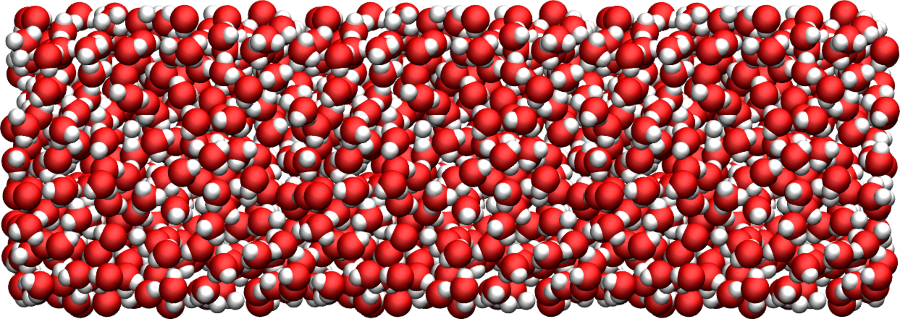
\includegraphics[width=\linewidth]{PEG-water}
\caption{Water reservoir after equilibration. Oxygen atoms are in red, and hydrogen atoms are in white.}
\label{fig:PEG-water}
\end{figure}

\begin{figure}
\centering
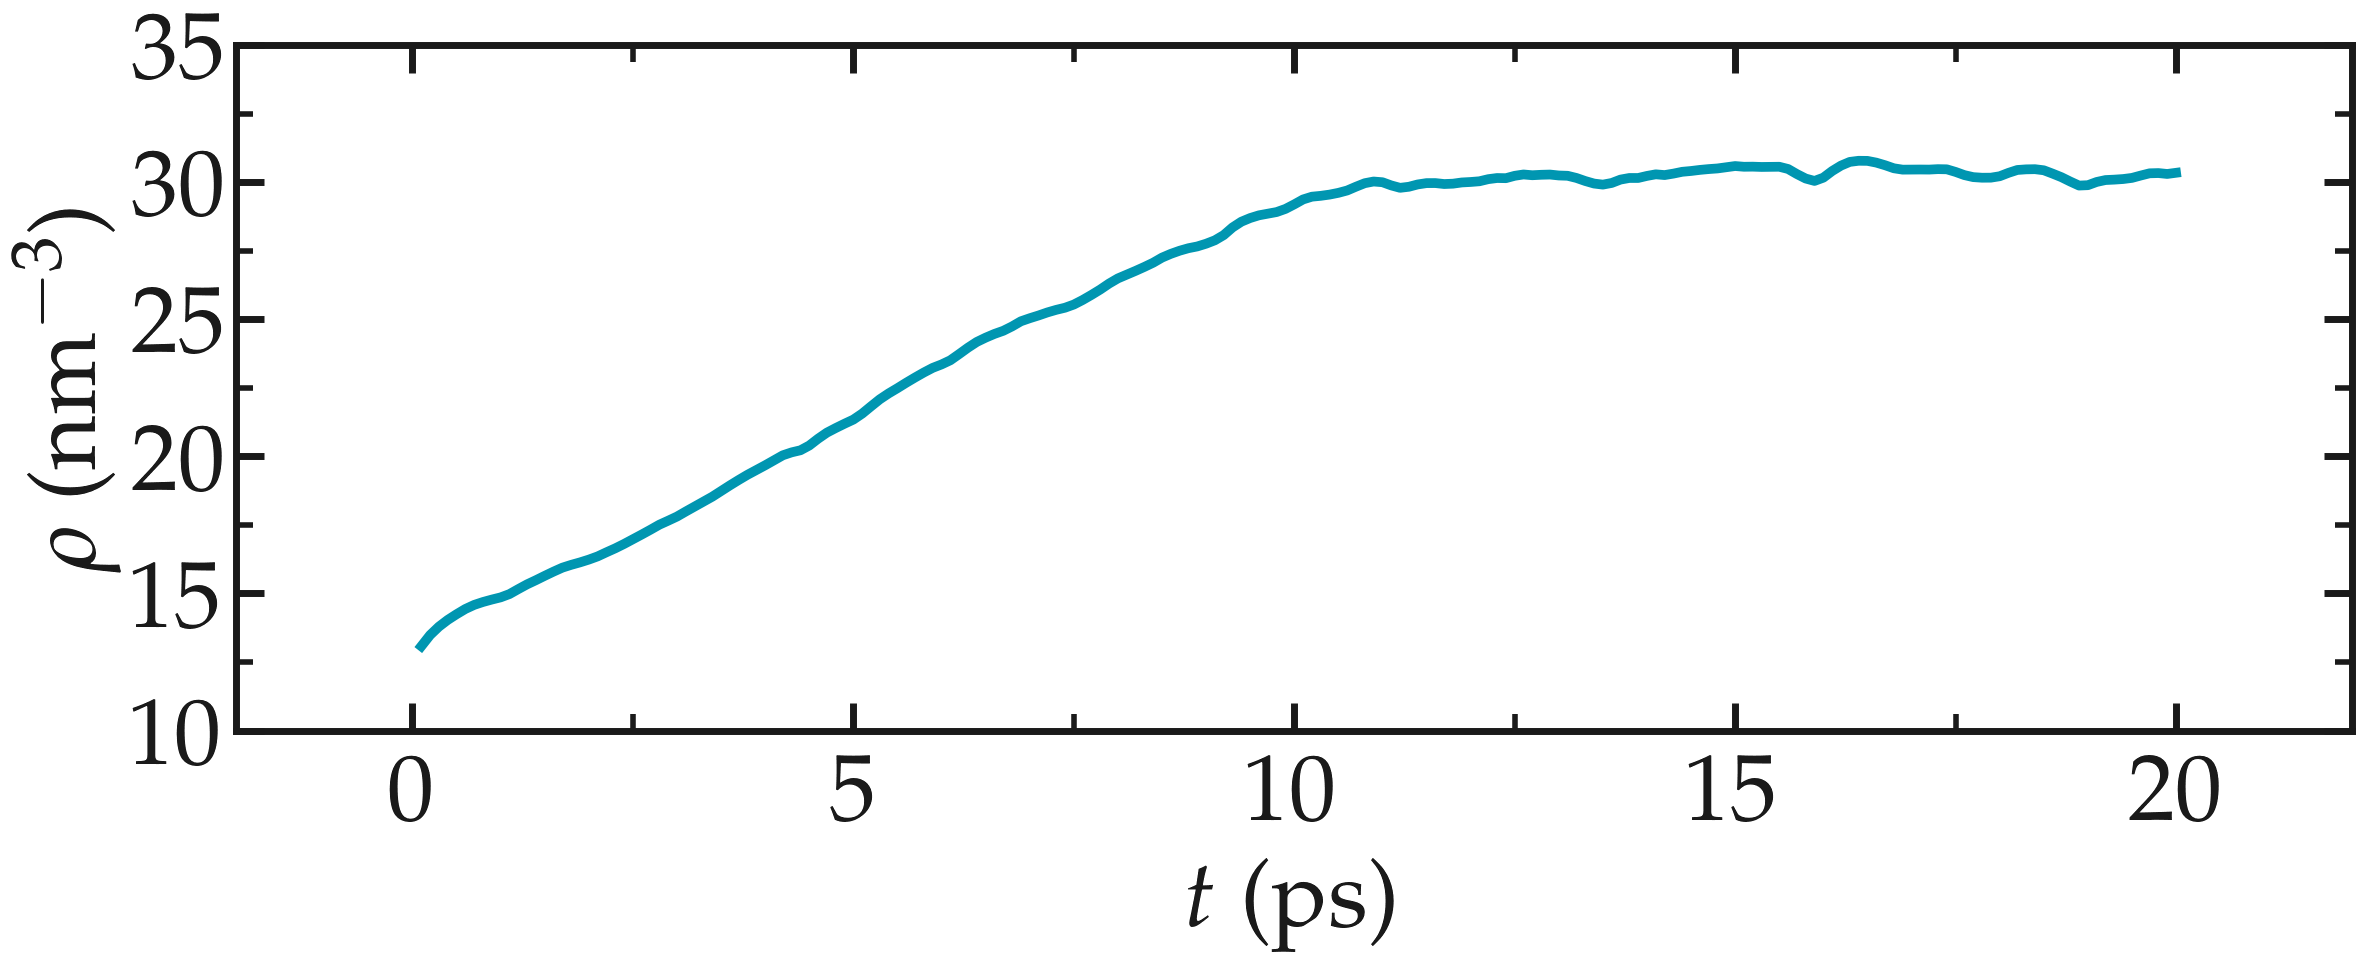
\includegraphics[width=\linewidth]{PEG-density}
\caption{Evolution of the density of water with time. The density $\rho$ reaches a plateau after $\approx 10\,\text{ps}$.}
\label{fig:PEG-density}
\end{figure}

\subsubsection{Solvating the PEG in water}
Once the water reservoir is equilibrated, we can safely include the PEG polymer in the water before performing the pull experiment on the polymer. The PEG molecule topology was downloaded from the ATB repository \cite{malde2011automated, oostenbrink2004biomolecular}. It has a formula $\text{C}_{28}\text{H}_{58}\text{O}_{15}$, and the parameters are taken from
the GROMOS 54A7 force field \cite{schmid2011definition}.

\begin{figure}
\centering
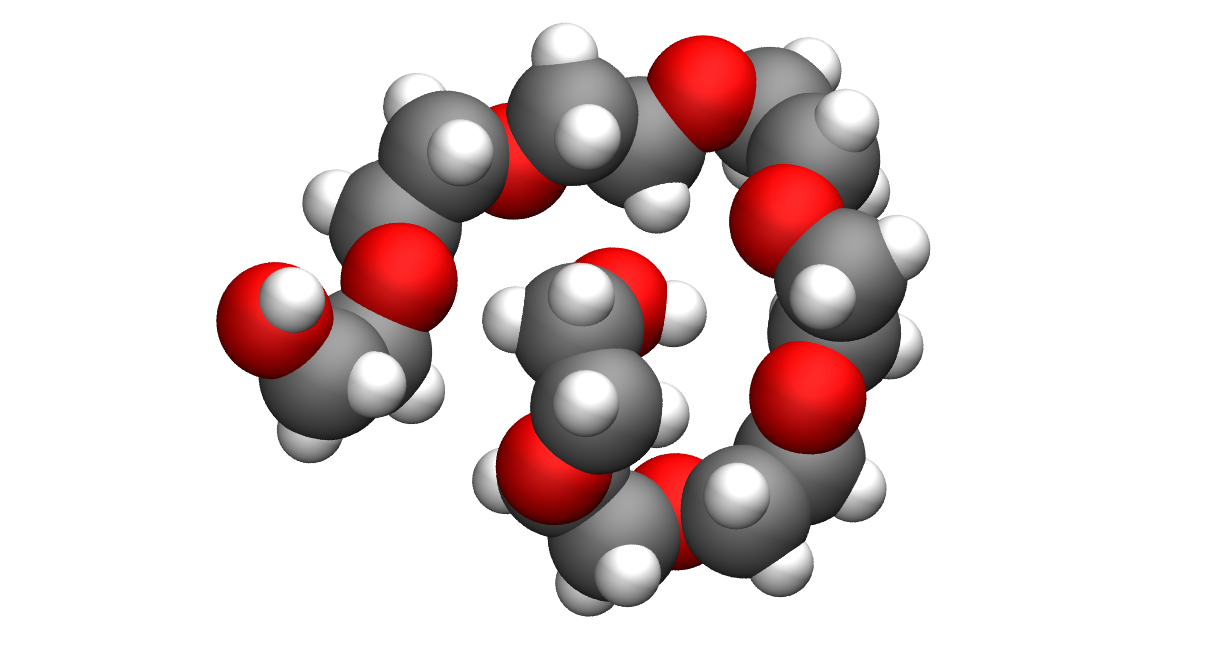
\includegraphics[width=\linewidth]{PEG-in-vacuum}
\caption{The PEG molecule in vacuum. The carbon atoms are in gray, the oxygen atoms in red, and the hydrogen atoms in white..}
\label{fig:PEG-in-vacuum}
\end{figure}

Create a second folder alongside \textit{pureH2O/} and call it \textit{mergePEGH2O/}. Create a new blank file in it,
call it \textit{input.lammps}. Within \textit{input.lammps}, copy the same first lines as previously:
\begin{verbatim}
units real
atom_style full
bond_style harmonic
angle_style harmonic
dihedral_style harmonic
pair_style lj/cut/coul/long 12
kspace_style pppm 1e-5
special_bonds lj 0.0 0.0 0.5 coul 0.0 0.0 1.0 &
    angle yes dihedral yes
\end{verbatim}
Then, import the previously generated data file \textit{H2O.data} as well as the \textit{PARM.lammps} file:
\begin{verbatim}
read_data ../pureH2O/H2O.data &
    extra/bond/per/atom 3 &
    extra/angle/per/atom 6 &
    extra/dihedral/per/atom 10 &
    extra/special/per/atom 14
include ../PARM.lammps
\end{verbatim}
Let us create a molecule called \textit{pegmol} from the molecule \href{https://lammpstutorials.github.io/lammpstutorials-inputs/level2/polymer-in-water/mergePEGH2O/PEG-GROMOS.mol}{template} for the PEG molecule, and let us create a single molecule in the middle of the box:
\begin{verbatim}
molecule pegmol PEG-GROMOS.mol
create_atoms 0 single 0 0 0 mol pegmol 454756
\end{verbatim}
Let us create 2 groups to differentiate the PEG from the H2O, by adding the following lines to \textit{input.lammps}:
\begin{verbatim}
group H2O type 8 9
group PEG type 1 2 3 4 5 6 7
\end{verbatim}
Water molecules that are overlapping with the PEG must be deleted to avoid future crashing. Add the following line to \textit{input.lammps}:
\begin{verbatim}
delete_atoms overlap 2.0 H2O PEG mol yes
\end{verbatim}
Here, the value of 2 Ångstroms for the overlap cutoff was fixed arbitrarily and can be chosen through trial and error. If the cutoff is too small, the simulation will crash. If the cutoff is too large, too many water molecules will unnecessarily be deleted.
Finally, let us use the \textit{fix npt} to control the temperature, as well as the pressure by allowing the box size to be rescaled along the \textit{x} axis:
\begin{verbatim}
fix mynpt all npt temp 300 300 100 x 1 1 1000
timestep 1.0
\end{verbatim}
Once more, let us dump the atom positions as well as the system temperature and volume:
\begin{verbatim}
dump mydmp all atom 100 dump.lammpstrj
thermo 100
variable mytemp equal temp
variable myvol equal vol
fix myat1 all ave/time 10 10 100 &
    v_mytemp file temperature.dat
fix myat2 all ave/time 10 10 100 &
    v_myvol file volume.dat
\end{verbatim}
Let us also print the total enthalpy:
\begin{verbatim}
variable myenthalpy equal enthalpy
fix myat3 all ave/time 10 10 100 &
    v_myenthalpy file enthalpy.dat
\end{verbatim}
Finally, let us perform a short equilibration and print the
final state in a data file. Add the following lines to the data file:
\begin{verbatim}
run 30000
write_data mix.data
\end{verbatim}
If you open the \textit{dump.lammpstrj} file using VMD, or have a look at the evolution of the volume in \textit{volume.dat},
you should see that the box dimension slightly evolves along \textit{x} to accommodate the new configuration.

\begin{figure}
\centering
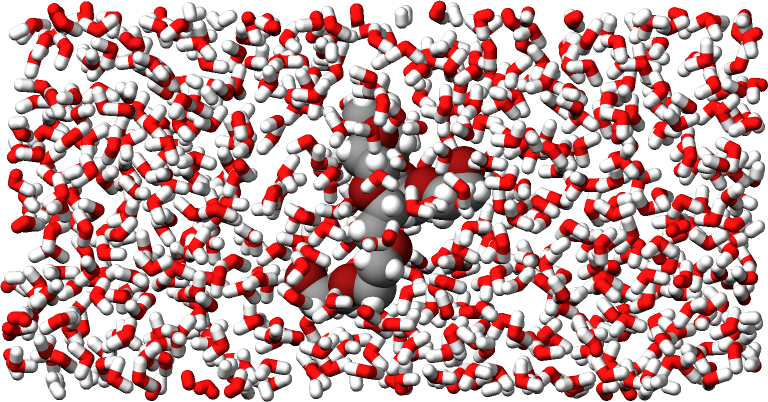
\includegraphics[width=\linewidth]{PEG-solvated}
\caption{A single PEG molecule in water. Water molecules are represented as a transparent continuum field for clarity.}
\label{fig:PEG-solvated}
\end{figure}

\subsubsection{Stretching the PEG molecule}
Here, a constant forcing is applied to the two ends of the PEG molecule until it stretches. Create a new folder next to the previously created folders, call it \textit{pullonPEG/}, and create a new input file in it called \textit{input.lammps}. First, let us create a variable \textit{f0} corresponding to the magnitude of the force we are going to apply. The force magnitude is chosen to be large enough to overcome the thermal agitation and the entropic contribution from both water
and PEG molecules (it was chosen by trial and error). Copy in the \textit{input.lammps} file:
\begin{verbatim}
variable f0 equal 5
\end{verbatim}
Note that $1\,\text{kcal/mol/Å}$ corresponds to $67.2\,\text{pN}$. Then, copy the same lines as previously:
\begin{verbatim}
units real
atom_style full
bond_style harmonic
angle_style harmonic
dihedral_style harmonic
pair_style lj/cut/coul/long 12
kspace_style pppm 1e-5
special_bonds lj 0.0 0.0 0.5 coul 0.0 0.0 1.0 &
    angle yes dihedral yes
\end{verbatim}
Start the simulation from the equilibrated PEG-water system and include again the parameter file by adding the following lines to the \textit{input.lammps}:
\begin{verbatim}
read_data ../mergePEGH2O/mix.data
include ../PARM.lammps
\end{verbatim}
Then, let us create 4 atom groups: H2O and PEG (as previously), as well as 2 groups containing only the 2 oxygen atoms of types 6 and 7, respectively. Atoms of types 6 and 7 correspond to the oxygen atoms located at the ends of the PEG molecule, which we are going to use to pull on the PEG molecule. Add the following lines to the \textit{input.lammps}:
\begin{verbatim}
group H2O type 8 9
group PEG type 1 2 3 4 5 6 7
group topull1 type 6
group topull2 type 7
\end{verbatim}
Add the following \textit{dump} command to the input to print the atom positions every 1000 steps:
\begin{verbatim}
dump mydmp all atom 1000 dump.lammpstrj
\end{verbatim}
Let us use a single Nosé-Hoover thermostat applied to all the atoms by adding the following lines to \textit{input.lammps}:
\begin{verbatim}
timestep 1.0
fix mynvt all nvt temp 300 300 100
\end{verbatim}
Let us also print the end-to-end distance of the PEG,
here defined as the distance between the groups \textit{topull1}
and \textit{topull2}, as well as the temperature of the system 
by adding the following lines to \textit{input.lammps}:
\begin{verbatim}
variable mytemp equal temp
fix myat1 all ave/time 10 10 100 &
    v_mytemp file output-temperature.dat
variable x1 equal xcm(topull1,x)
variable x2 equal xcm(topull2,x)
variable y1 equal xcm(topull1,y)
variable y2 equal xcm(topull2,y)
variable z1 equal xcm(topull1,z)
variable z2 equal xcm(topull2,z)
variable delta_r equal &
    sqrt((v_x1-v_x2)^2+(v_y1-v_y2)^2+(v_z1-v_z2)^2)
fix myat2 all ave/time 10 10 100 v_delta_r &
    file output-end-to-end-distance.dat
thermo 1000
\end{verbatim}
Finally, let us simulate 30 picoseconds without any external forcing:
\begin{verbatim}
run 30000
\end{verbatim}
This first run serves as a benchmark to quantify the changes induced by the forcing. Then, let us apply a forcing on the 2 oxygen atoms using two \textit{add$\_$force} commands, and run for an extra 30 ps:
\begin{verbatim}
fix myaf1 topull1 addforce ${f0} 0 0
fix myaf2 topull2 addforce -${f0} 0 0
run 30000
\end{verbatim}
If you open the \textit{dump.lammpstrj} file using \textit{VMD}, you should see that the PEG molecule eventually aligns in the direction of the force (Fig.\,\ref{fig:PEG-in-water}). The evolution of the end-to-end distance over time shows the PEG adjusting to the external forcing (Fig.\,\ref{fig:PEG-distance}).

\begin{figure}
\centering
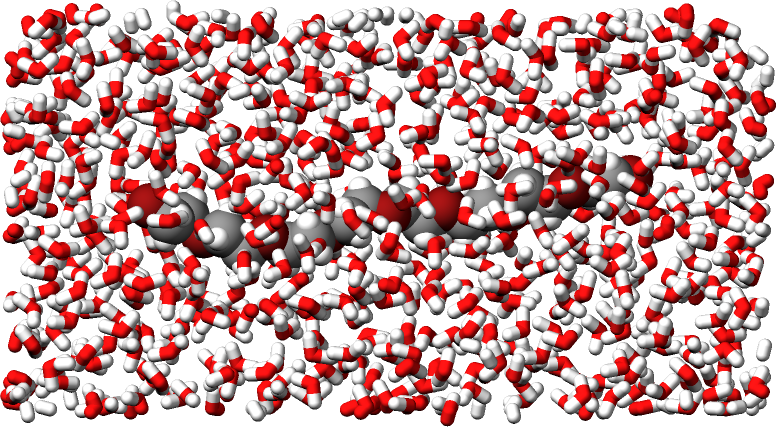
\includegraphics[width=\linewidth]{PEG-in-water}
\caption{PEG molecule stretched along the \textit{x} direction in water. Water molecules are represented as a transparent continuum field for clarity.}
\label{fig:PEG-in-water}
\end{figure}

\begin{figure}
\centering
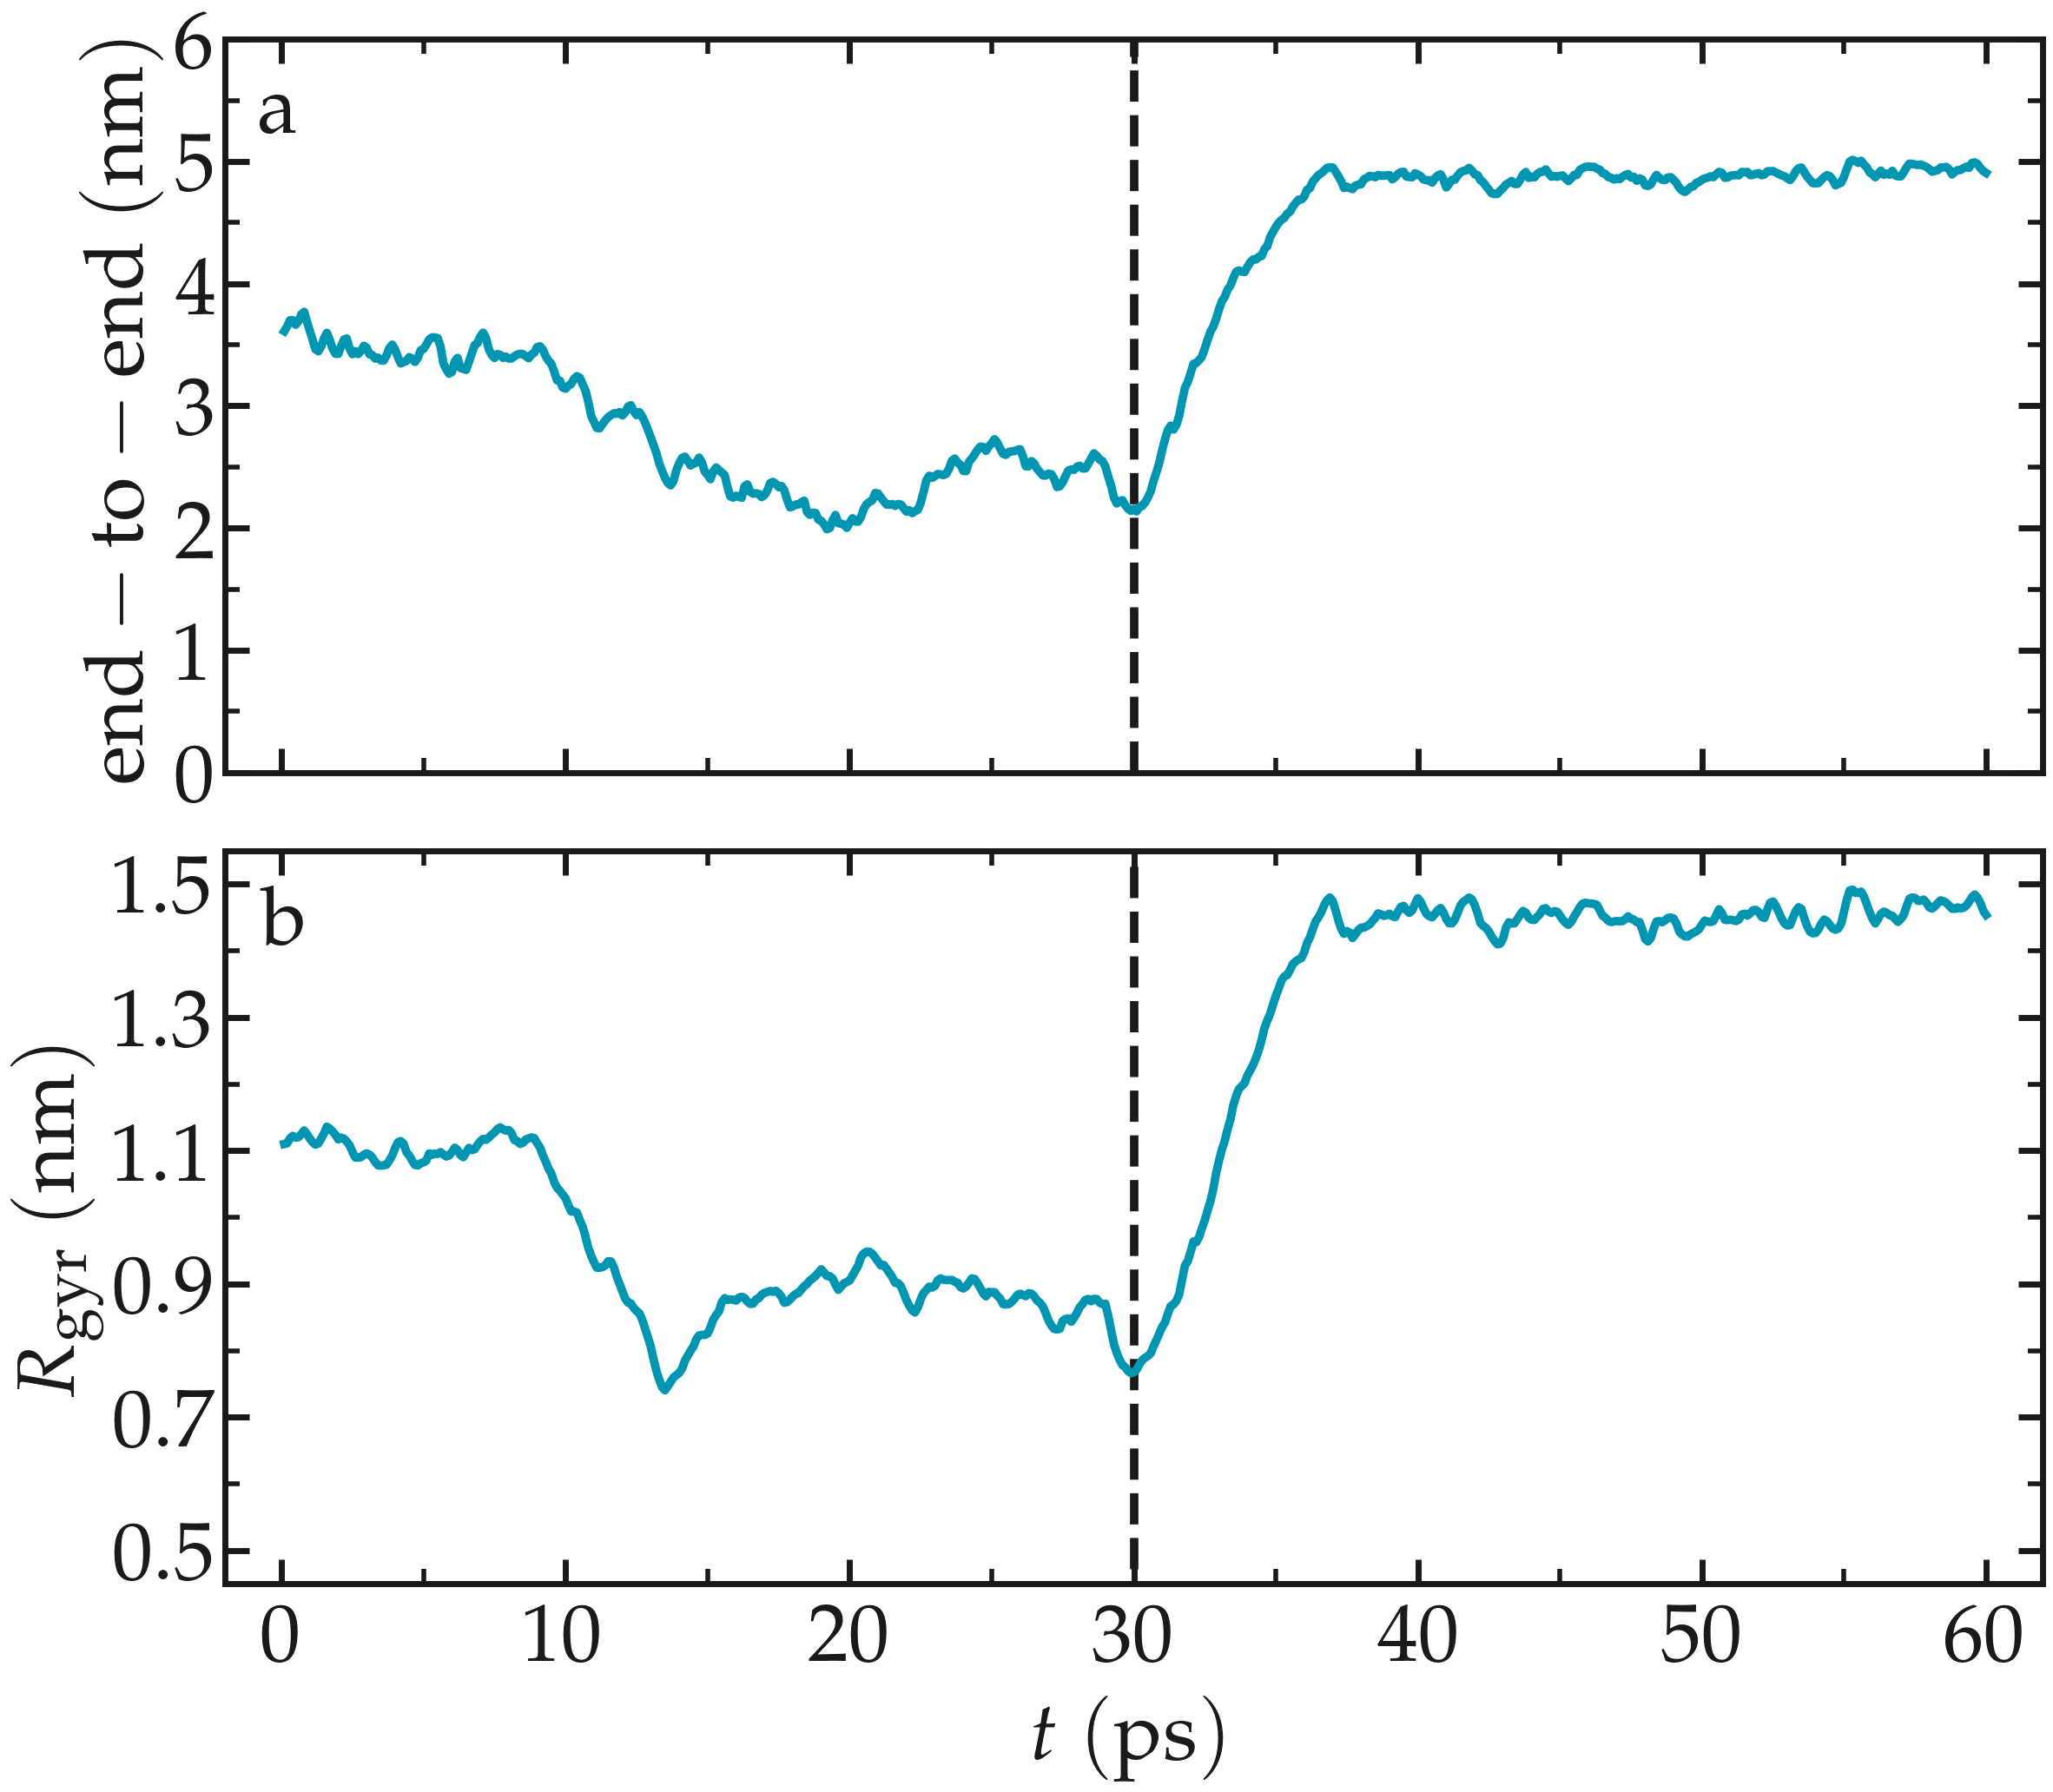
\includegraphics[width=\linewidth]{PEG-distance}
\caption{Evolution of the end-to-end distance of the PEG molecule with time. The forcing starts at $t = 30$ ps.}
\label{fig:PEG-distance}
\end{figure}

\subsection{Tutorial 4: Nanosheared electrolyte}
\label{sheared-confined-label}

\begin{figure}
{\centering
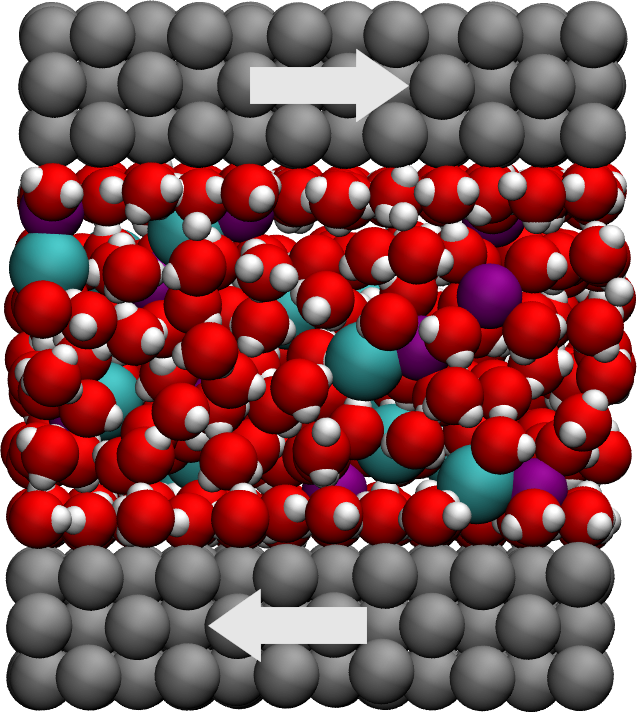
\includegraphics[width=0.55\linewidth]{NANOSHEAR}
\caption{Snapshot of the electrolyte nano-confined in a slit pore.}}
\label{fig:NANOSHEAR}
\end{figure}

The objective of this tutorial is to simulate an electrolyte nanoconfined and sheared by two walls (Fig.\,\ref{fig:NANOSHEAR}). Some properties of the sheared fluid, such as its density and velocity profiles, will be extracted. This tutorial illustrates some key aspects of
combining a fluid and a solid in the same simulation. A major difference with the previous tutorial, \hyperref[all-atoms-label]{Polymer in water}, is that here a rigid four points water model named TIP4P is used \cite{abascal2005general}. TIP4P is one of the most common water models due to its high accuracy.

\subsubsection{System preparation}
The fluid and walls must first be generated, and then equilibrated at reasonable temperature and pressure.

\paragraph{System generation}
Create a new folder called \textit{systemcreation/}. Within \textit{systemcreation/}, open a blank file called \textit{input.lammps}, and copy the following lines into it:
\begin{verbatim}
units real
atom_style full
bond_style harmonic
angle_style harmonic
pair_style lj/cut/tip4p/long 1 2 1 1 0.1546 12.0
kspace_style pppm/tip4p 1.0e-4
\end{verbatim}
These lines are used to define the most basic parameters, including the \textit{atom}, \textit{bond}, and \textit{angle} styles, as well as interaction potential. Here \textit{lj/cut/tip4p/long} imposes a Lennard Jones potential with a cut-off at $12\,\text{$\text{\AA{}}$}$ and a long-range Coulomb potential. So far, the commands are relatively similar to the 
previous tutorial (\hyperref[all-atoms-label]{Polymer in water}), with two major differences; the use of \textit{lj/cut/tip4p/long} and \textit{pppm/tip4p}, instead of \textit{lj/cut/coul/long} and pppm. These two tip4p-specific commands allow us to model a four-point water molecule without explicitly defining the fourth massless atom \textit{M}. The value of 
$0.1546\,\text{$\text{\AA{}}$}$ corresponds to the \textit{O-M} distance and is given by the water model. Here, TIP4P-2005 is used \cite{abascal2005general}.

Let us create the box by adding the following lines to \textit{input.lammps}:
\begin{verbatim}
lattice fcc 4.04
region box block -3 3 -3 3 -7 7
create_box 5 box &
bond/types 1 &
angle/types 1 &
extra/bond/per/atom 2 &
extra/angle/per/atom 1 &
extra/special/per/atom 2
\end{verbatim}
The \textit{lattice} command defines the unit cell. Here, the face-centered cubic (fcc) lattice with a scale factor of
4.04 has been chosen for the future positioning of the atoms of the walls. The \textit{region} command defines a geometric
region of space. By choosing \textit{xlo=-3} and \textit{xhi=3}, and because we have previously chosen a lattice with a scale
factor of 4.04, the region box extends from -12.12 Å to 12.12 Å along the $x$ direction. The \textit{create$\_$box} command creates a simulation box with 5 types of atoms: the oxygen and hydrogen of the water molecules, the two ions ($\text{Na}^+$,
$\text{Cl}^-$), and the atom of the walls. The \textit{create$\_$box} command extends over 6 lines thanks to the $\&$ character. The second and third lines are used to indicate that the simulation contains 1 type of bond and 1 type of angle (both required by the water molecule). The parameters for these bond and angle constraints will be given later. The
three last lines are for memory allocation. Now, we can add atoms to the system. First, let us create two sub-regions corresponding respectively to the two solid walls, and create a larger region from the union of the two regions. Then, let us create atoms of type 5 (the wall) within the two regions. Add the following lines to \textit{input.lammps}:
\begin{verbatim}
region rbotwall block -3 3 -3 3 -4 -3
region rtopwall block -3 3 -3 3 3 4
region rwall union 2 rbotwall rtopwall
create_atoms 5 region rwall
\end{verbatim}
Atoms will be placed in the positions of the previously defined lattice, thus forming fcc solids. In order to add the water molecules, first download the \href{https://lammpstutorials.github.io/lammpstutorials-inputs/level2/nanosheared-electrolyte/systemcreation/RigidH2O.txt}{molecule template} and place it within \textit{systemcreation/}. The template contains all the
necessary information concerning the water molecule, such as atom positions, bonds, and angles. Add the following lines to \textit{input.lammps}:
\begin{verbatim}
region rliquid block INF INF INF INF -2 2
molecule h2omol RigidH2O.txt
create_atoms 0 region rliquid mol h2omol 482793
\end{verbatim}
Within the last four lines, a \textit{region} named \textit{rliquid} for depositing the water molecules are created based on the last defined lattice, which is \textit{fcc 4.04}. The \textit{molecule} command opens up the molecule template named
\textit{RigidH2O.txt}, and names the associated molecule \textit{h2omol}. Molecules are created on the \textit{fcc 4.04} lattice by the \textit{create$\_$atoms} command. The first parameter is '0', meaning that the atom ids from the \textit{RigidH2O.txt} file will be used. The number \textit{482793} is a seed that is required by LAMMPS, it can be any positive integer. Finally, let us create 30 ions (15 $\text{Na}^+$ and 15 $\text{Cl}^-$) in between the water molecules, by adding the following commands to \textit{input.lammps}:
\begin{verbatim}
create_atoms 3 random 15 52802 rliquid &
    overlap 0.3 maxtry 500
create_atoms 4 random 15 90182 rliquid &
    overlap 0.3 maxtry 500
set type 3 charge 1
set type 4 charge -1
\end{verbatim}
Each \textit{create$\_$atoms} command will add 15 ions at random positions within the \textit{rliquid} region, ensuring that there is no \textit{overlap} with existing molecules. Feel free to increase or decrease the salt concentration by changing the number of desired ions. To keep the system charge neutral, always insert the same number of $\text{Na}^+$ and $\text{Cl}^-$, unless there are other charges in the system. The charges of the newly added ions are specified by the two \textit{set} commands.

Before starting the simulation, we still need to define the parameters of the simulation: the mass of the 5 atom types (O, H, $\text{Na}^+$, $\text{Cl}^-$, and wall), the pairwise interaction parameters (here, the parameters for the Lennard-Jones potential), and the bond and angle parameters. Copy the following line into \textit{input.lammps}:
\begin{verbatim}
include ../PARM.lammps
include ../GROUP.lammps
\end{verbatim}
Create a new text file, call it \textit{PARM.lammps}, and copy it next to the \textit{systemcreation/} folder. Copy the following lines into PARM.lammps:
\begin{verbatim}
mass 1 15.9994 # water
mass 2 1.008 # water
mass 3 28.990 # ion
mass 4 35.453 # ion
mass 5 26.9815 # wall

pair_coeff 1 1 0.185199 3.1589 
pair_coeff 2 2 0.0 1.0 # water
pair_coeff 3 3 0.04690 2.4299
pair_coeff 4 4 0.1500 4.04470
pair_coeff 5 5 11.697 2.574
pair_coeff 1 5 0.4 2.86645

bond_coeff 1 0 0.9572

angle_coeff 1 0 104.52
\end{verbatim}
Each \textit{mass} command assigns a mass in grams/mole to an atom type. Each \textit{pair$\_$coeff} assigns respectively the depth of the LJ potential (in Kcal/mole), and the distance (in Ångstrom) at which the particle-particle potential energy is 0.

As already seen in previous tutorials, and with the important exception of \textit{pair$\_$coeff 1 5}, only pairwise interaction between atoms of identical types were assigned. By default, LAMMPS calculates the pair coefficients for the interactions between atoms of different types (i and j) by using geometrical average: $\epsilon_{ij} = (\epsilon_{ii} + \epsilon_{jj})/2$,  $\sigma_{ij} = (\sigma_{ii} + \sigma_{jj})/2.$ Other rules for cross coefficients can be set with the \textit{pair$\_$modify} command, but for the sake of simplicity, the default option is kept here. By default, the value of $\epsilon_\text{1-5} = 5.941\,\text{kcal/mol}$ would be extremely high (compared to the water-water energy $\epsilon_\text{1-1} = 0.185199\,\text{kcal/mol}$), which would make the surface extremely hydrophilic. The walls were made less hydrophilic by reducing the  LJ energy of interaction $\epsilon_\text{1-5}$. The \textit{bond$\_$coeff}, which is here used for the O-H bond of the water molecule, sets both the energy of the harmonic potential and the equilibrium distance in Ångstrom. The value is \textit{0} for the energy because we are going to use a rigid model for the water molecule. The shape of the molecule will be preserved later by the \textit{shake} algorithm. Similarly, the angle coefficient here for the H-O-H angle of the water molecule sets the energy of the harmonic potential (also 0) and the equilibrium angle is in degree.

Let us also create another file called \textit{GROUP.lammps} next to \textit{PARM.lammps}, and copy the following lines into it:
\begin{verbatim}
group H2O type 1 2
group Na type 3
group Cl type 4
group ions union Na Cl
group fluid union H2O ions

group wall type 5
region rtop block INF INF INF INF 0 INF
region rbot block INF INF INF INF INF 0
group top region rtop
group bot region rbot
group walltop intersect wall top
group wallbot intersect wall bot
\end{verbatim}
To avoid high density and pressure, let us add the following lines to \textit{input.lammps} to delete a few of the water molecules:
\begin{verbatim}
delete_atoms random fraction 0.15 yes &
    H2O NULL 482793 mol yes
\end{verbatim}
Finally, add the following lines to \textit{input.lammps}:
\begin{verbatim}
run 0

write_data system.data
write_dump all atom dump.lammpstrj
\end{verbatim}
With \textit{run 0}, the simulation will run for 0 steps, which is enough for creating the system and saving the final state. The \textit{write$\_$data} creates a file named \textit{system.data} containing all the information required to restart the
simulation from the final configuration generated by this input file. The \textit{write$\_$dump} command prints the final
positions of the atoms, and can be opened with VMD to visualize the system. Run the \textit{input.lammps} file using LAMMPS. Always check that your system has been correctly created by looking at the periodic images. Atomic defects may occur at the boundary (Fig.\,\ref{fig:NANOSHEAR-system}).

\begin{figure}
\centering
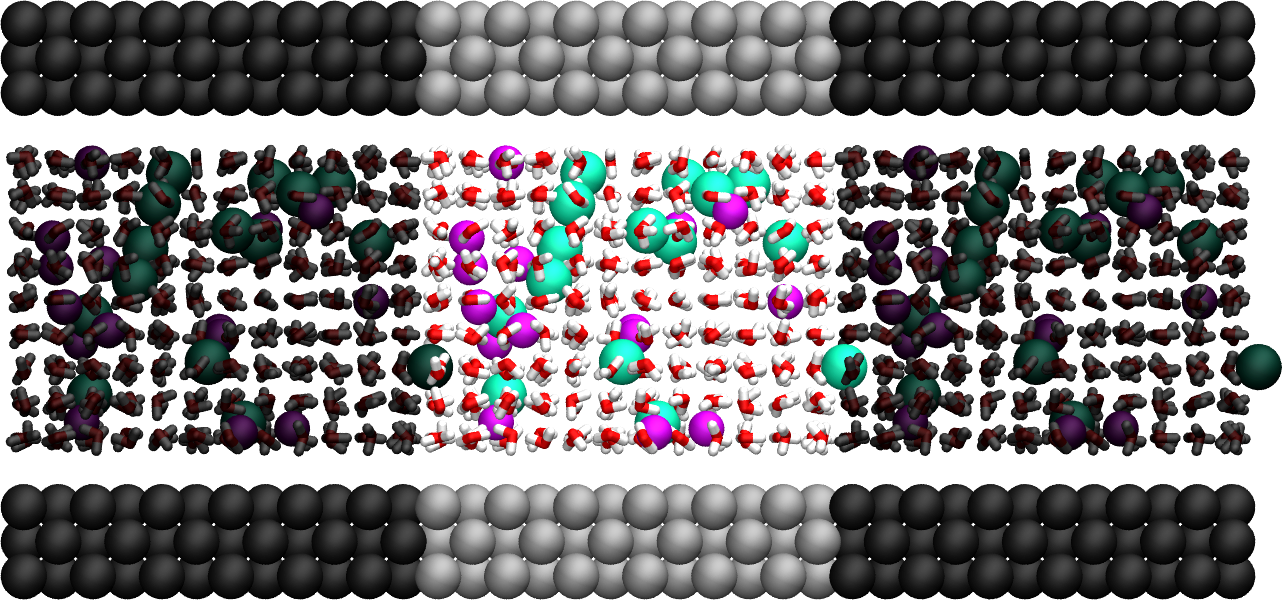
\includegraphics[width=\linewidth]{NANOSHEAR-system}
\caption{Side view of the system. Periodic images are represented in darker colors. Water molecules are in red and white, $\text{Na}^+$ ions in purple, $\text{Cl}^-$ ions in lime, and wall atoms in gray. Note the absence of atomic defect at the cell boundaries.}
\label{fig:NANOSHEAR-system}
\end{figure}

\paragraph{Energy minimization}
Let us move the atoms and place them in more energetically favorable positions before starting the simulation. Let us call this step \textit{energy minimization}, although it is not a conventional \textit{minimization} as done for instance
in the first tutorial; \hyperref[lennard-jones-label]{Lennard Jones fluid}. To perform this energy minimization, let us
create a new folder named \textit{minimization/} next to \textit{systemcreation/}, and create a new input file named \textit{input.lammps} in it. Copy the following lines in \textit{input.lammps}:
\begin{verbatim}
boundary p p p
units real
atom_style full
bond_style harmonic
angle_style harmonic
pair_style lj/cut/tip4p/long 1 2 1 1 0.1546 12.0
kspace_style pppm/tip4p 1.0e-4

read_data ../systemcreation/system.data

include ../PARM.lammps
include ../GROUP.lammps
\end{verbatim}
The only difference with the previous input is that, instead of creating a new box and new atoms, we open the previously created file \textit{system.data} located in \textit{systemcreation/}. The file \textit{system.data} contains the definition of the simulation box and the positions of the atoms. Now, let us create a first simulation step using a relatively small 
timestep ($0.5\,\text{fs}$), as well as a low temperature of $T = 1\,\text{K}$:
\begin{verbatim}
fix mynve fluid nve/limit 0.1
fix myber fluid temp/berendsen 1 1 100
fix myshk H2O shake 1.0e-4 200 0 b 1 a 1
timestep 0.5
\end{verbatim}
Just like \textit{fix nve}, the fix \textit{nve/limit} performs constant NVE integration to update positions and velocities of the atoms at each timestep, but also limits the maximum distance atoms can travel at each timestep. Here, only the fluid molecules and ions will move. The \textit{fix temp/berendsen} rescales the velocities of the atoms to force the temperature of the system to reach the desired value of 1 K, and the shake algorithm is used in order to maintain the shape of the water molecules. Let us also print the atom positions in a \textit{.lammpstrj} file by adding the following line to \textit{input.lammps}:
\begin{verbatim}
dump mydmp all atom 1000 dump.lammpstrj
thermo 200
\end{verbatim}
Finally, let us run for 4000 steps. Add the  following lines into \textit{input.lammps}:
\begin{verbatim}
run 4000
\end{verbatim}
In order to better equilibrate the system, let us perform two additional steps with a larger timestep and a larger imposed temperature:
\begin{verbatim}
fix myber fluid temp/berendsen 300 300 100
timestep 1.0

run 4000

unfix mynve
fix mynve fluid nve

run 4000

write_data system.data
\end{verbatim}
For the last of the 3 steps, fix \textit{nve} is used instead of \textit{nve/limit}, which will allow for a better relaxation of the atom positions. When running the \textit{input.lammps} file with LAMMPS, you should see that the total energy of the system decreases during the first of the 3 steps, before re-increasing a little after the temperature is increased from 1 to $300\,\text{K}$ (Fig.\,\ref{fig:NANOSHEAR-minimization}). If you look at the trajectory using VMD, you will see some of the atoms, in particular, the ones that were
initially in problematic positions. 

\begin{figure}
\centering
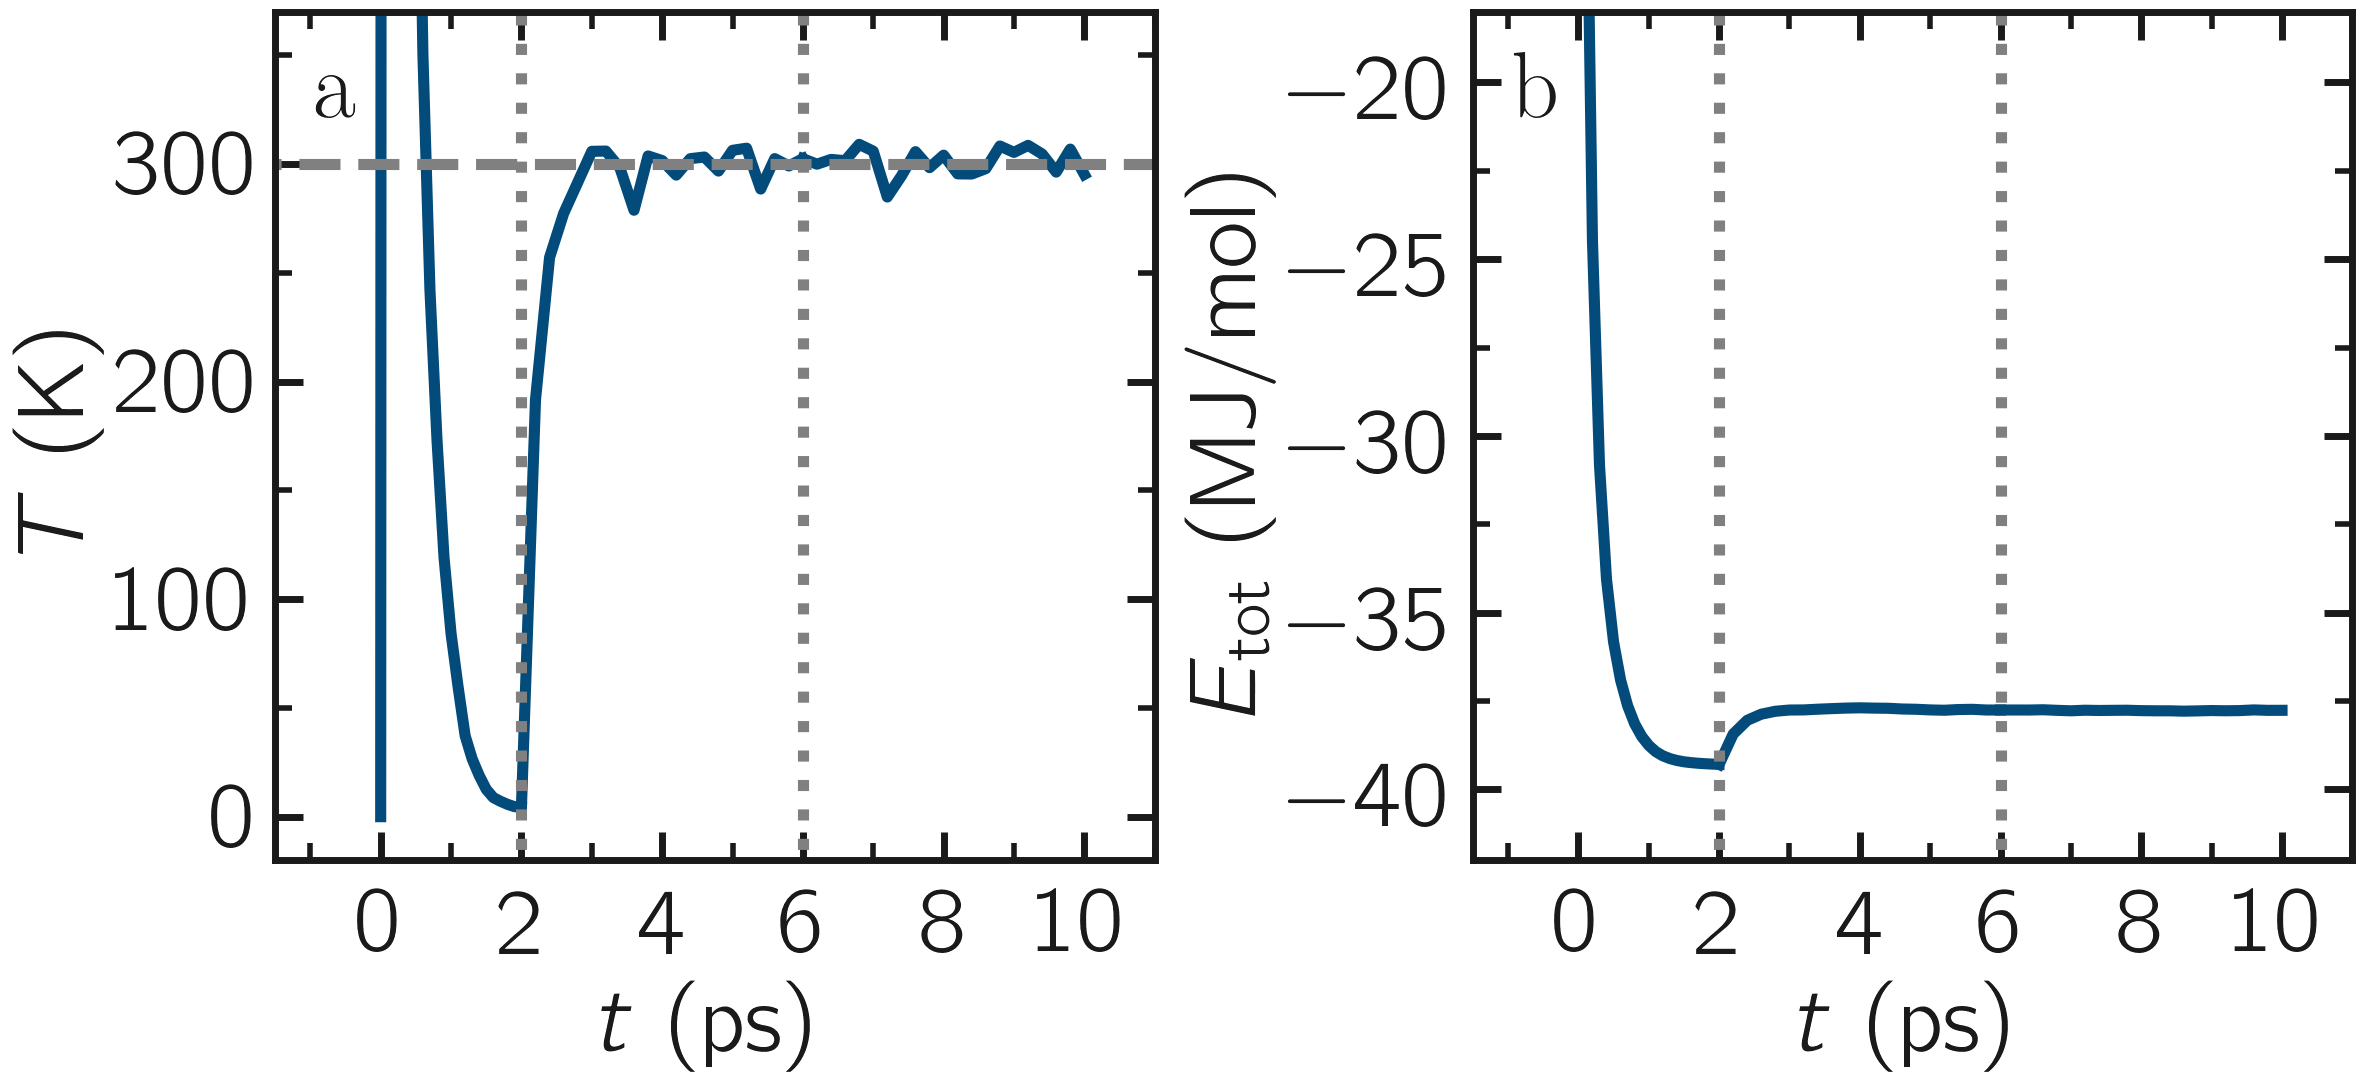
\includegraphics[width=\linewidth]{NANOSHEAR-minimization}
\caption{Energy as a function of time extracted from the log file using \textit{Python} and \textit{lammps$\_$logfile}.}
\label{fig:NANOSHEAR-minimization}
\end{figure}

\paragraph{System equilibration}
Now, let us equilibrate further the entire system by letting both fluid and piston relax at ambient temperature. Create a new folder called \textit{equilibration/} next to the previously created folders, and create a new \textit{input.lammps} file in it. Add the following lines into \textit{input.lammps}:
\begin{verbatim}
boundary p p p
units real
atom_style full
bond_style harmonic
angle_style harmonic
pair_style lj/cut/tip4p/long 1 2 1 1 0.1546 12.0
kspace_style pppm/tip4p 1.0e-4

read_data ../minimization/system.data

include ../PARM.lammps
include ../GROUP.lammps
\end{verbatim}
Finally, let us complete the \textit{input.lammps} file:
\begin{verbatim}
fix mynve all nve
fix myber all temp/berendsen 300 300 100
fix myshk H2O shake 1.0e-4 200 0 b 1 a 1
fix myrct all recenter NULL NULL 0
timestep 1.0
\end{verbatim}
The fix \textit{recenter} has no influence on the dynamics, but will keep the system in the center of the box, which makes the
visualization easier. Then, add the following lines to \textit{input.lammps} for the trajectory visualization and output:
\begin{verbatim}
dump mydmp all atom 1000 dump.lammpstrj
thermo 500
variable walltopz equal xcm(walltop,z)
variable wallbotz equal xcm(wallbot,z)
variable deltaz equal v_walltopz-v_wallbotz
fix myat1 all ave/time 100 1 100 v_deltaz &
    file interwall_distance.dat
\end{verbatim}
The first two variables extract the centers of mass of the two walls. Then, the \textit{deltaz} variable is used to calculate the distance between the two variables \textit{walltopz} and \textit{wallbotz}, i.e. the distance between the two walls.

Finally, let us add the \textit{run} command: 
\begin{verbatim}
run 30000
write_data system.data  
\end{verbatim}
Run the \textit{input.lammps} file using LAMMPS. As seen from the data printed by \textit{fix myat1}, the distance $\delta_z$ between the two walls reduces until it reaches an equilibrium value (Fig.\,\ref{fig:NANOSHEAR-equilibration}). Note that it is generally recommended to run longer equilibration. Here, for instance, the slowest process in the system is probably the ionic diffusion. Therefore the equilibration should in principle be longer than the time
the ions need to diffuse over the size of the pore ($\approx 1.2\,\text{nm}$), i.e. of the order of half a nanosecond.

\begin{figure}
\centering
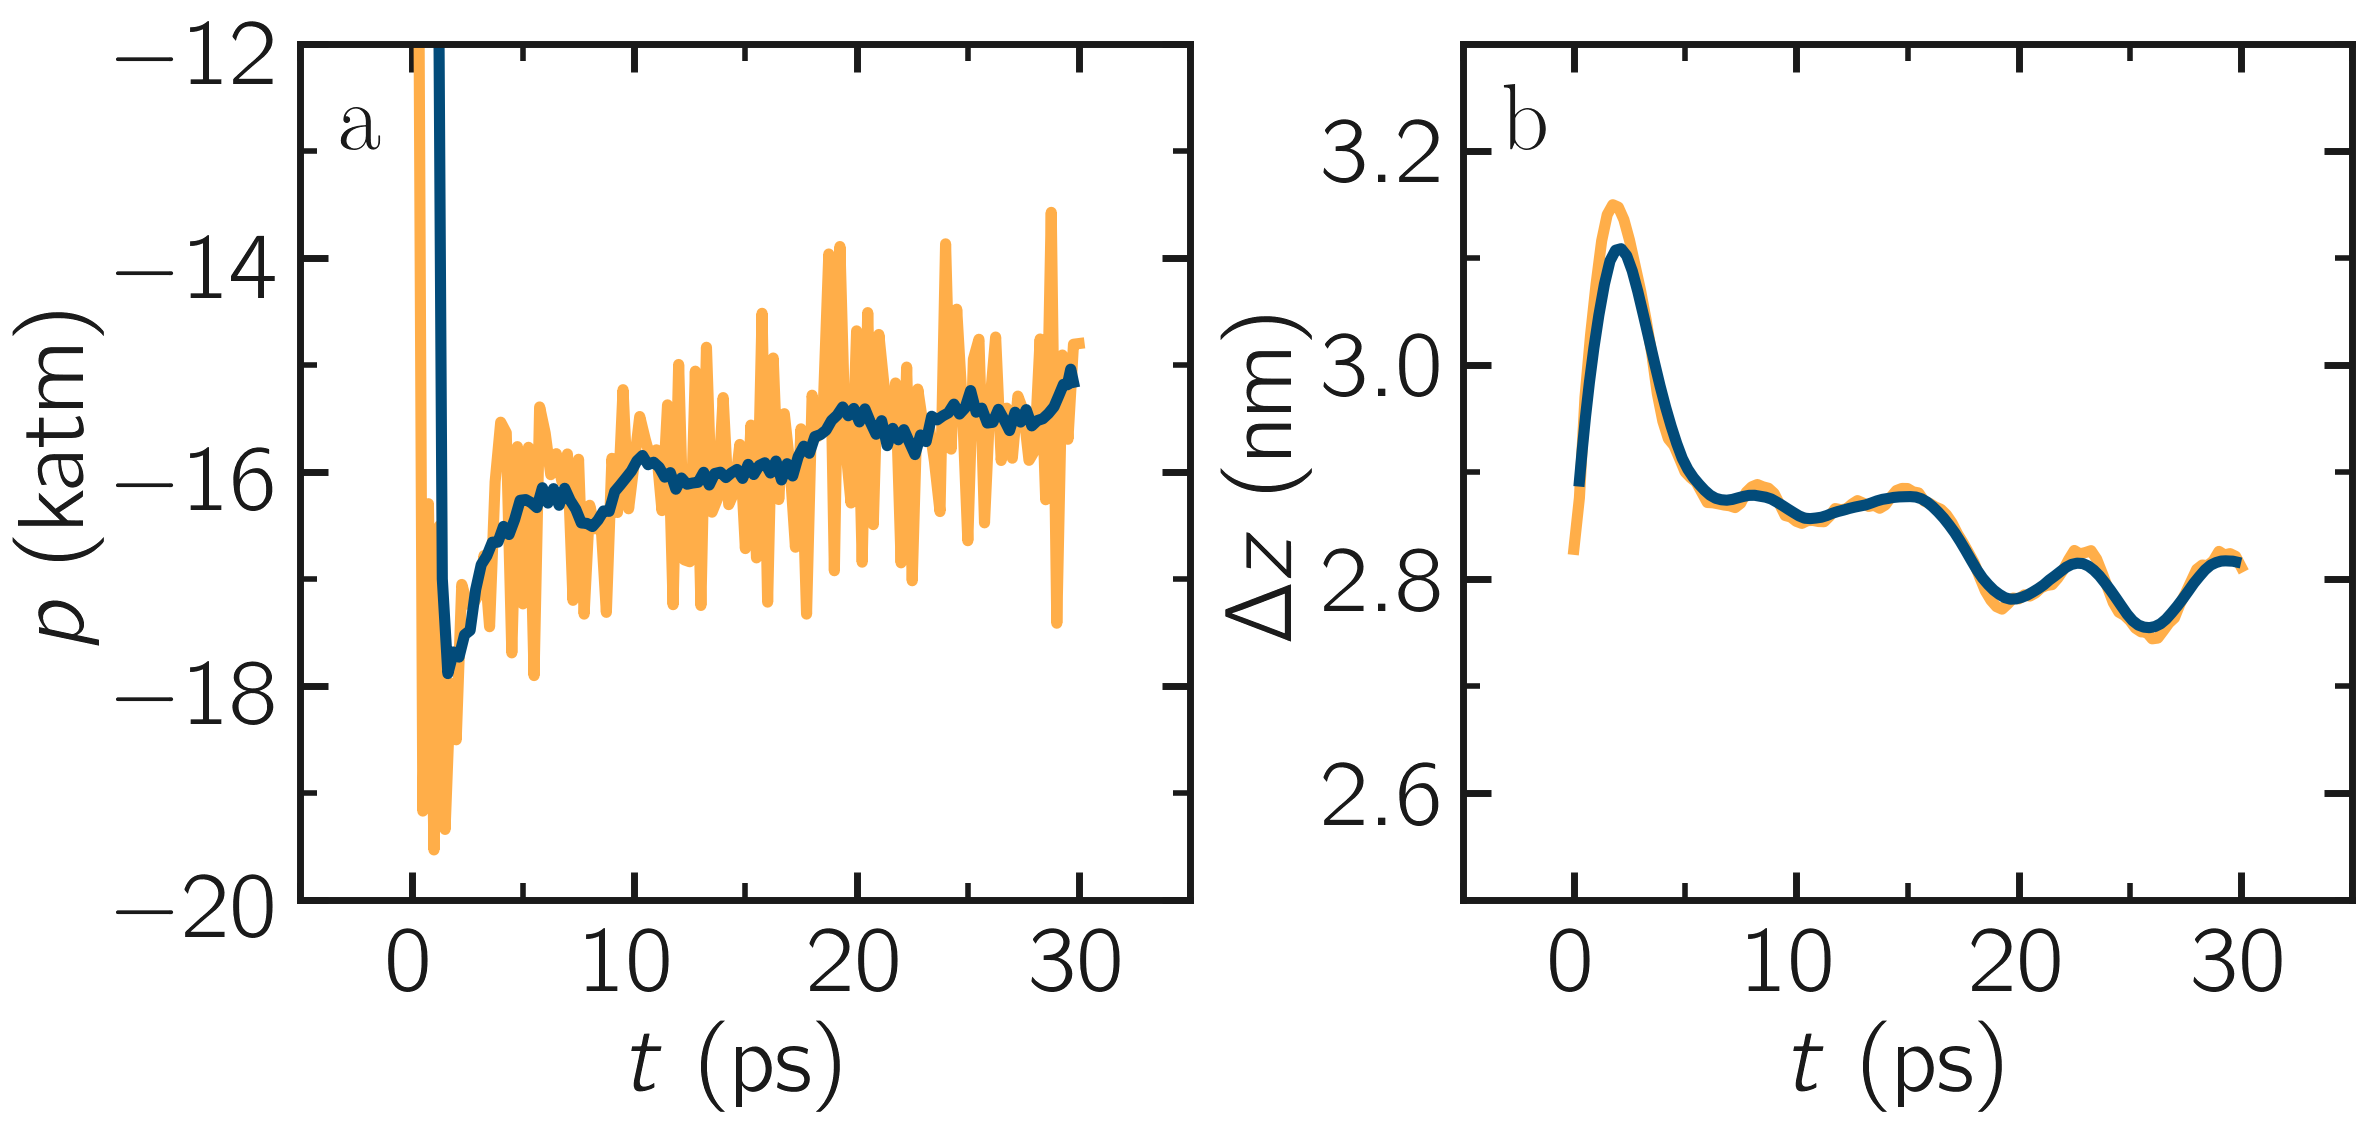
\includegraphics[width=\linewidth]{NANOSHEAR-equilibration}
\caption{Distance between the walls as a function of time. After a few picoseconds, the distance between the two walls equilibrates near its final value.}
\label{fig:NANOSHEAR-equilibration}
\end{figure}

\subsubsection{Imposed shearing}

From the equilibrated configuration, let us impose a laterial motion to the two walls and shear the electrolyte.
In a new folder called \textit{shearing/}, create a new \textit{input.lammps} file that starts like the previous ones:
\begin{verbatim}
boundary p p p
units real
atom_style full
bond_style harmonic
angle_style harmonic
pair_style lj/cut/tip4p/long 1 2 1 1 0.1546 12.0
kspace_style pppm/tip4p 1.0e-4
\end{verbatim}
Let us import the previously equilibrated data, include the parameter and group files, and then deal with the dynamics of the system.
\begin{verbatim}
read_data ../equilibration/system.data

include ../PARM.lammps
include ../GROUP.lammps

fix mynve all nve
compute Tfluid fluid temp/partial 0 1 1
fix myber1 fluid temp/berendsen 300 300 100
fix_modify myber1 temp Tfluid
compute Twall wall temp/partial 0 1 1
fix myber2 wall temp/berendsen 300 300 100
fix_modify myber2 temp Twall
fix myshk H2O shake 1.0e-4 200 0 b 1 a 1
fix myrct all recenter NULL NULL 0
\end{verbatim}
One difference here is that two thermostats are used, one for the fluid (\textit{myber1}) and one for the solid (\textit{myber2}). The use of \textit{fix$\_$modify} together with \textit{compute} ensures that the right temperature value is used by the thermostats. The use of temperature \textit{compute} with \textit{temp/partial 0 1 1} is meant to exclude the \textit{x} coordinate from the thermalization, which is important since a large velocity will be imposed along \textit{x}. 

Then, let us impose the velocity of the two walls  by adding the following command to \textit{input.lammps}:
\begin{verbatim}
fix mysf1 walltop setforce 0 NULL NULL
fix mysf2 wallbot setforce 0 NULL NULL
velocity wallbot set -2e-4 NULL NULL
velocity walltop set 2e-4 NULL NULL
\end{verbatim}
The \textit{setforce} commands cancel the forces on \textit{walltop} and \textit{wallbot}, respectively. Therefore the atoms of the two groups do not experience any force from the rest of the system. In the absence of force acting on those atoms, they will conserve their initial velocity. The \textit{velocity} commands act only once and impose the velocity of the atoms of the groups \textit{wallbot} and \textit{walltop}, respectively.

Finally, let us dump the atom positions, extract the velocity profiles using several \textit{ave/chunk} commands, extract the
force applied on the walls, and then run for $200\,\text{ps}$ Add the following lines to \textit{input.lammps}:
\begin{verbatim}
dump mydmp all atom 5000 dump.lammpstrj
thermo 500
thermo_modify temp Tfluid

compute cc1 H2O chunk/atom bin/1d z 0.0 1.0
compute cc2 wall chunk/atom bin/1d z 0.0 1.0
compute cc3 ions chunk/atom bin/1d z 0.0 1.0

fix myac1 H2O ave/chunk 10 15000 200000 &
cc1 density/mass vx file water.profile_1A.dat
fix myac2 wall ave/chunk 10 15000 200000 &
cc2 density/mass vx file wall.profile_1A.dat
fix myac3 ions ave/chunk 10 15000 200000 &
cc3 density/mass vx file ions.profile_1A.dat

fix myat1 all ave/time 10 100 1000 f_mysf1[1] &
    f_mysf2[1] file forces.dat

timestep 1.0
run 200000
write_data system.data
\end{verbatim}
Here, a binning of $1\,\text{Å}$ is used. For smoother profiles, you can reduce its value. The averaged velocity and density profiles of the fluid can be plotted (Figs.\ref{fig:NANOSHEAR-velocity}-\ref{fig:NANOSHEAR-density}). As expected here, the velocity of the fluid is found to increase linearly along $z$.

\begin{figure}
\centering
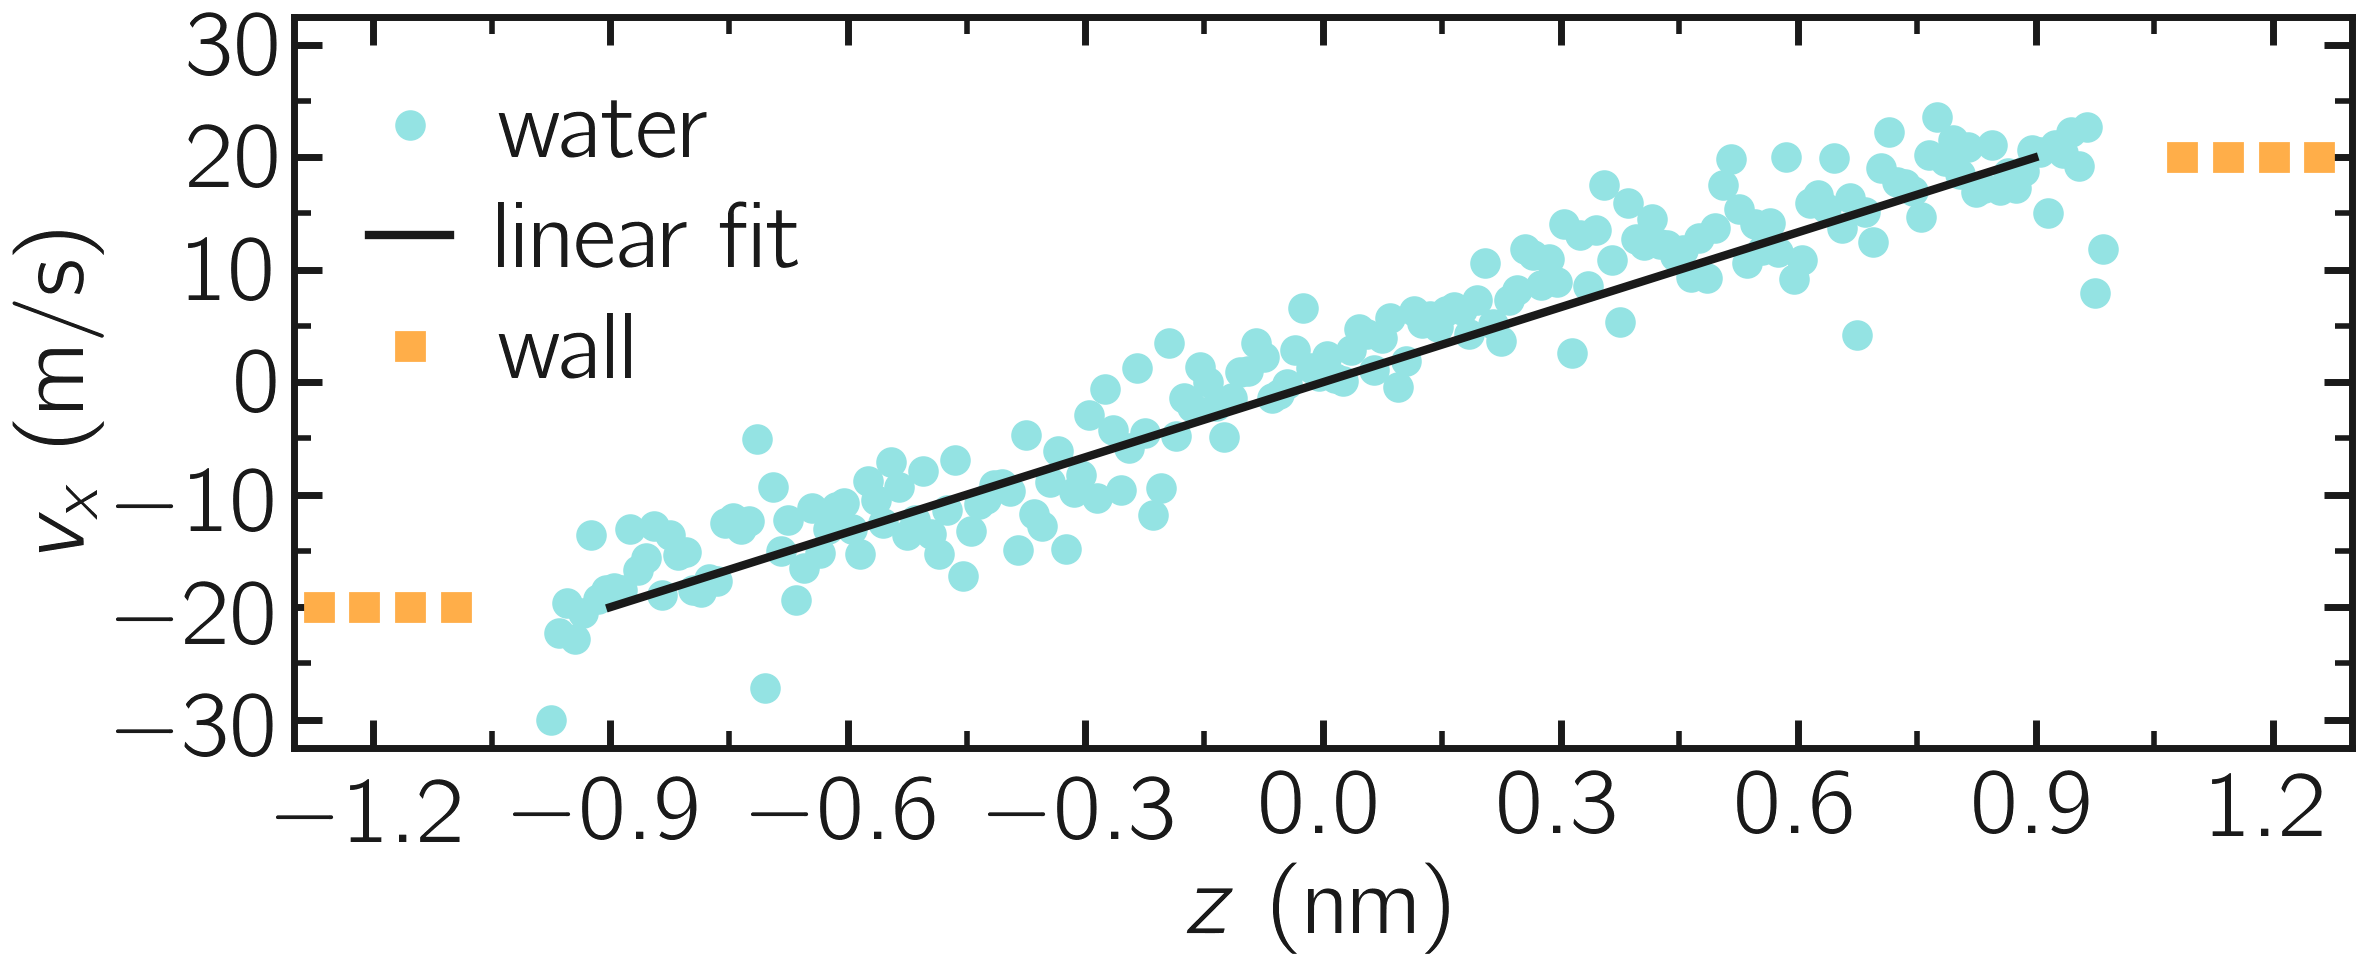
\includegraphics[width=\linewidth]{NANOSHEAR-velocity}
\caption{Velocity profiles for water molecules, ions and walls along the \textit{z} axis. The line is a linear fit assuming that the pore size is $h = 1.8\,\text{nm}$.}
\label{fig:NANOSHEAR-velocity}
\end{figure}

\begin{figure}
\centering
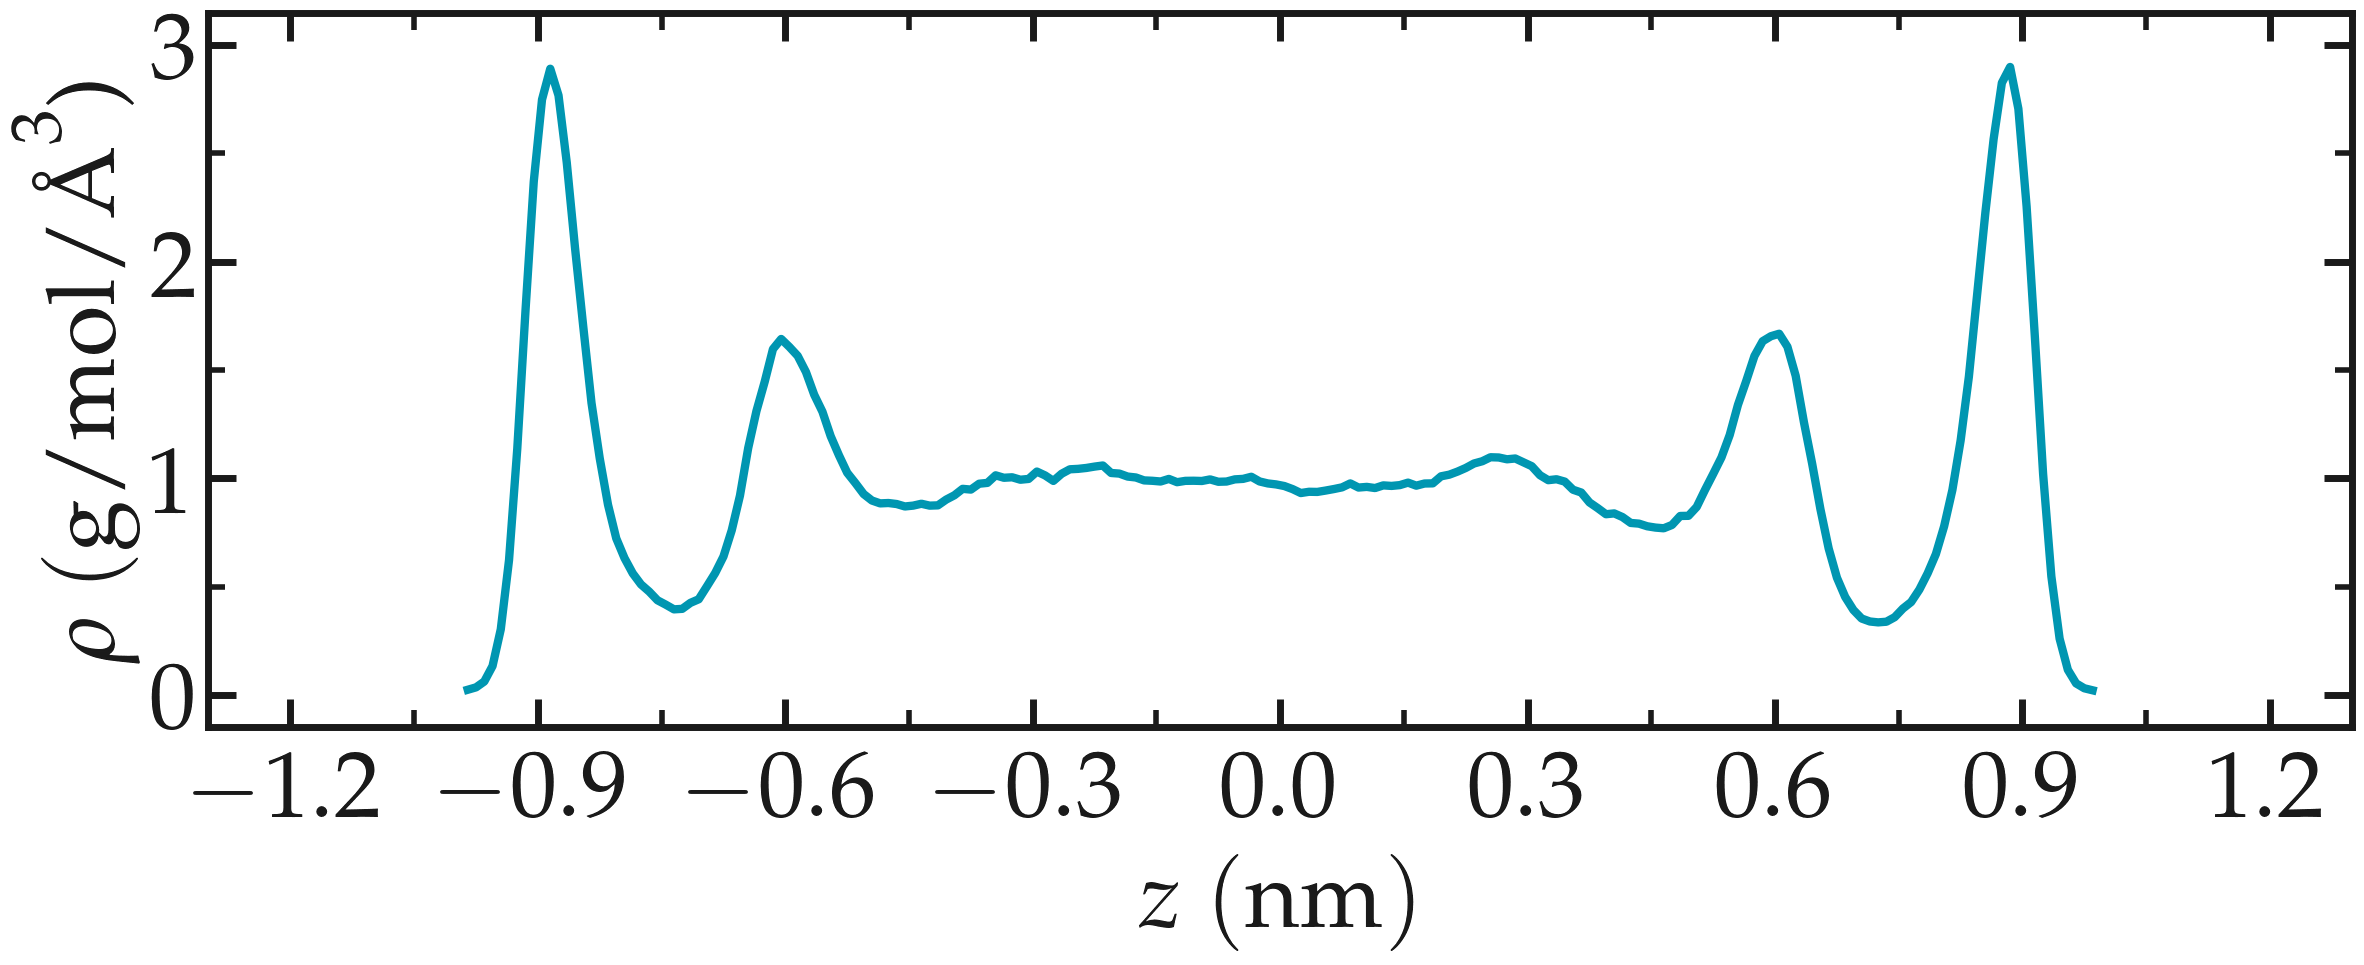
\includegraphics[width=\linewidth]{NANOSHEAR-density}
\caption{Water density $\rho$ profile along the \textit{z} axis.}
\label{fig:NANOSHEAR-density}
\end{figure}

From the force applied by the fluid on the solid, one can extract the stress within the fluid, which allows one to
measure its viscosity $\dot{\eta}$ according to: $\eta = \tau / \dot{\gamma}$ where $\tau$ is the stress applied by the fluid on the shearing wall, and $\dot{\gamma}$ the shear rate (which is imposed here) \cite{gravelle2021violations}. Here the shear rate is approximatively $\dot{\gamma} = 16 \cdot 10^9\,\text{s}^{-1}$, and using a surface area of $A = 6 \cdot 10^{-18}\,\text{m}^2$, one gets an estimate for the shear viscosity for the confined fluid of $\eta = 6.6\,\text{mPa.s}$. The viscosity calculated at such a high shear rate may differ from the expected \textit{bulk} value. In general, it is recommended to use a lower value for the shear rate. Note that for lower shear rates, the ratio of noise-to-signal is larger, and longer simulations are needed. Another important point is that the viscosity of a fluid next to a solid surface is typically larger than in bulk due to interaction with the walls. Therefore, one expects the present simulation to return a viscosity that is slightly larger than what would be measured in the absence of a wall.















\section*{Author Contributions}

SG conceived and wrote all the online tutorials and underlying Sphinx
documentation for \href{https://lammpstutorials.github.io}{lammpstutorials.github.io}.

\section*{Potentially Conflicting Interests}

There are no conflicting interests to declare.

\section*{Funding Information}

S.G. acknowledges funding from the European Union's Horizon 2020 research and
innovation programme under the Marie Skłodowska-Curie grant agreement N$^\circ\;101065060$.

\section*{Author Information}
\makeorcid

\bibliography{journal-article}

%%%%%%%%%%%%%%%%%%%%%%%%%%%%%%%%%%%%%%%%%%%%%%%%%%%%%%%%%%%%
%%% APPENDICES
%%%%%%%%%%%%%%%%%%%%%%%%%%%%%%%%%%%%%%%%%%%%%%%%%%%%%%%%%%%%

%\appendix


\end{document}
